
\chapter{\enginline{3.} ಯೋಗಾಭ್ಯಾಸದ ವೈಜ್ಞಾನಿಕ ಅಧ್ಯಯನ}

ಎಲ್ಲ ತರದ ಯೋಗಾಭ್ಯಾಸಗಳು ದೇಹ ಮತ್ತು ಮನಸ್ಸುಗಳ ನಿಕಟ ಸಂಬಂಧವನ್ನು ಬೆಳೆಸುತ್ತವೆ. ಮಾತ್ರವಲ್ಲದೆ ಅವೆರಡರ ಸಮಗ್ರ ಸಮನ್ವಯವನ್ನು ಉಳಿಸಿ ಕೊಳ್ಳಲೂ ಸಾಧಕವಾಗುತ್ತವೆ. ಅದರಿಂದಾಗಿ, ಜೀವನ ಜಂಝಾಟದಿಂದ ಒದಗುವ ಮಾನಸಿಕ ತುಮುಲಗಳ ದುಷ್ಪರಿಣಾಮಗಳು ಕಡಿಮೆಯಾಗುತ್ತವೆ.

ಹೀಗೆಲ್ಲ ಹೇಳಲಾಗುತ್ತಿದೆಯಾದರೂ, ಈ ವಿಷಯವನ್ನು ವೈಜ್ಞಾನಿಕವಾಗಿ ಅಧ್ಯಯನ ಮಾಡಿ ಖಡಾಖಂಡಿತವಾಗಿ ಹೇಳುವುದು ಇಂದಿಗೆ ಬೇಕಾಗಿದೆ. ಯೋಗಾ ಭ್ಯಾಸದ ಪ್ರಭಾವದಿಂದ ದೇಹ ಮತ್ತು ಮನಸ್ಸಿನ ಮೇಲೆ ಆಗುವ ಶಾರೀರಿಕ, ಮಾನಸಿಕ ಮತ್ತು ಜೀವರಾಸಾಯನಿಕ ಬದಲಾವಣೆಗಳನ್ನು ಪರೀಕ್ಷಿಸಿ ಅಳತೆಮಾಡಿ ಹೇಳಬೇಕಾಗುತ್ತದೆ. ಅದಕ್ಕಿರುವ ವಿವಿಧ ವೈಜ್ಞಾನಿಕ ಉಪಕರಣಗಳನ್ನೂ ಬಳಸ ಬೇಕಾಗುತ್ತದೆ.

ಅಂತಹ ವೈಜ್ಞಾನಿಕ ಅಧ್ಯಯನವನ್ನು ಎರಡು ತರದಲ್ಲಿ ಮಾಡಬರುತ್ತದೆ. \enginline{(1)} ಯೋಗಾಭ್ಯಾಸ ನಿಪುಣರಾದ ಸಮರ್ಥ ಯೋಗಿಗಳ ದೇಹಮನಸ್ಸಾಮರ್ಥ್ಯದ ಸಮಗ್ರ ಪರೀಕ್ಷೆಯಿಂದ ನಡೆಸಬಹುದಾಗಿದೆ. ಹಾಗೆಯೇ \enginline{(2)} ಸಾಮಾನ್ಯ ಸ್ವಯಂ ಸೇವಕರಿಗೆ ಯೋಗಾಭ್ಯಾಸ ಮಾಡಕಲಿಸಿ ಅವರ ದೇಹ ಮನಸ್ಸುಗಳಲ್ಲಾಗುವ ಬದಲಾವಣೆಗಳ ಅಧ್ಯಯನಗೈದು ತಿಳಿಯಬಹುದಾಗಿದೆ.

ಡಾ. ಆನಂದ ಮತ್ತು ಡಾ. ಚಿನ ಎಂಬ ವೈದ್ಯ ವಿಜ್ಞಾನಿಗಳಿಬ್ಬರು ಮೊತ್ತ ಮೊದಲಾಗಿ ಮೂರು ಮಂದಿ ಸಮರ್ಥಯೋಗಿಗಳ ಯೋಗಸಾಮರ್ಥ್ಯವನ್ನು ವೈಜ್ಞಾನಿಕವಾಗಿ ಅಧ್ಯಯನ ಮಾಡಿದರು. ಆ ಮೂವರು ಯೋಗಿಗಳು ಬೇಕಾದಾಗ ತಮ್ಮ ಹೃದಯ ಬಡಿತವನ್ನು ತಡೆದಿಟ್ಟುಕೊಳ್ಳಬಲ್ಲೆವೆಂದು ಹೇಳುತ್ತಿದ್ದರು. ಅದರ ಸತ್ಯಾಸತ್ಯತೆಯನ್ನು ಇ.ಸಿ.ಜಿ., ಇ.ಇ.ಜಿ. ಮತ್ತು \enginline{Finger plathymograph—} ಮುಂತಾದ ಉಪಕರಣಗಳನ್ನು ಬಳಸಿಕೊಂಡು ಪರೀಕ್ಷಿಸಿ ನೋಡಿದರು. ಡಾ~। ವಾಗೀರ್, ಡಾ~। ಬಾಗ್ಚಿ ಮತ್ತು ಡಾ~। ಆನಂದ—ಇವರು ಇದೇ ವಿಷಯದಲ್ಲಿ ಮತ್ತೊಂದು ಅಧ್ಯಯನವನ್ನೂ ನಡೆಸಿದರು. ಡಾ~। ಆನಂದ್, ಡಾ~। ಚಿನ, ಮತ್ತು ಡಾ~। ಬಲದೇವಸಿಂಗ್​—ಇವರು, ಯೋಗಿಯೊಬ್ಬನನ್ನು \enginline{10' × 4'} ಗಾತ್ರದ ಗಾಳಿ ಹೋಗದಂತೆ ಬೆಸುಗೆ ಹಾಕಿ ಮುದ್ರೆಗೈದ ಕಬ್ಬಿಣ ಮತ್ತು ಗಾಜಿನ ಪೆಟ್ಟಿಗೆಯೊಳಗೆ \enginline{8–10} ಘಂಟೆಗಳ ಕಾಲ ಕೂರಿಸಿ, ಆತನ ಆಮ್ಲಜನಕ \enginline{(02)} ಸೇವನೆ, ಮತ್ತು ಇಂಗಾಲಾಮ್ಲದ \enginline{(CO2)} ಬಿಡುಗಡೆ—ಮುಂತಾದ ಜೀವದ್ರವ್ಯಬದಲಾವಣೆಗಳನ್ನು ಅಧ್ಯಯನ ಮಾಡಿದರು. ಡಾ~। ಕೊಠಾರಿ ಅವರು \enginline{48} ಘಂಟೆಗಳ ಕಾಲ ನೆಲದಡಿಯ ಹೊಂಡದಲ್ಲಿದ್ದ ಯೋಗಿಯ ಜೀವದ್ರವ್ಯ ಬದಲಾವಣೆಗಳ ಅಧ್ಯಯನವನ್ನೂ ನಡೆಸಿದರು.

ಈ ಎಲ್ಲ ತರದ ಅಧ್ಯಯನಗಳಿಂದ ಸಮರ್ಥ ಯೋಗಿಯು ದೇಹದ ಸಾಮಾನ್ಯ ಮಾನವನ ಅಧೀನದಲ್ಲಿ ಇಲ್ಲದ ಸ್ವತಂತ್ರ ವ್ಯವಹಾರಗಳಾದ ಎದೆ ಬಡಿತ, ಶ್ವಾಸೋಚ್ಛ್ವಾಸ ಮುಂತಾದುವನ್ನು ಇಷ್ಟಬಂದಂತೆ ಹಿಡಿದಿಟ್ಟುಕೊಳ್ಳಲು ಸಮರ್ಥನಾಗಿರುತ್ತಾನೆ; ಕೆಲವೆಲ್ಲ ಉಭಯ (ಜಲ, ನೆಲ) ಜೀವಿಗಳು ತಮ್ಮ ನಿಶ್ಚೇಷ್ಟಾವಸ್ಥೆಯ ಕಾಲದಲ್ಲಿ ಮಾಡಿಕೊಳ್ಳುವಂತೆ, ಬೇಕಾದ ತರದಲ್ಲಿ ಉಸಿರಾಟವೇ ಮೊದಲಾದ ನಮ್ಮ ಶಕ್ತ್ಯತೀತ ದೇಹವ್ಯಾಪಾರಗಳನ್ನು ತಡೆದಿಟ್ಟುಕೊಳ್ಳಲೂ ಯೋಗಿ ಸಮರ್ಥನಾಗಿರುತ್ತಾನೆ; ಸ್ವಾತಂತ್ರ ನರವೂಹ್ಯಗಳ ಕ್ರಿಯೆಗಳನ್ನು ಸಹ ಹಿಡಿತಕ್ಕೆ ತಂದುಕೊಂಡು ಅದ್ಭುತಶಕ್ತಿ ಪ್ರದರ್ಶಿಸಲು ಶಕ್ತನಾಗಿರುತ್ತಾನೆ; ಎಂದು ಮೊದಲಾದ ಅಂಶಗಳು ವೈದ್ಯ ವಿಜ್ಞಾನಿಗಳ ಅಧ್ಯಯನದಿಂದ ತಿಳಿದುಬಂದವು.

ಡಾ~। ಆನಂದ್, ಡಾ~। ಚಿನ ಮತ್ತು ಡಾ~। ಬಲದೇವಸಿಂಗ್​—ಇವರು ಸಮಾಧಿ ಸ್ಥಿತಿಯಲ್ಲಿರುವ ನಾಲ್ವರು ಯೋಗಿಗಳ ಮಿದುಳಿನ ಪ್ರರೂಪದ ವಿಸ್ತೃತ ಅಧ್ಯಯನ ವನ್ನು ಮಸ್ತಿಷ್ಕ ವಿದ್ಯುಲ್ಲೇಖಕ \enginline{(E.E.G.)} ಉಪಕರಣದ ಸಹಾಯದಿಂದ ನಡೆಸಿ ದರು. ಅವರಲ್ಲಿಬ್ಬರು ಯೋಗಿಗಳನ್ನು ಮಿತಿಮೀರಿದ ಬೆಳಕು ಬೀರುವ ದ್ಯುತ್ಯಾತ್ಮಕ ಉದ್ದೀಪಕಕ್ಕೂ, ದೊಡ್ಡ ಶಬ್ದಗೈಯುವ ಶ್ರವಣಾತ್ಮಕ ಉದ್ದೀಪಕಕ್ಕೂ ಗುರಿಪಡಿಸಲಾಯಿತು. ಇನ್ನಿಬ್ಬರನ್ನು— \enginline{4º C} ಡಿಗ್ರಿಯಷ್ಟು ಹಿಮಶೀತ ನೀರಿನಲ್ಲಿ \enginline{45} ರಿಂದ \enginline{55} ನಿಮಿಷಗಳವರೆಗೆ ಕೈಯನ್ನದ್ದಿ ನೋವುಂಟುಮಾಡುವ ಉದ್ದೀಪಕಕ್ಕೆ ಗುರಿಪಡಿಸ ಲಾಯಿತು.

ಹೀಗೆ ಮಾಡಿದರೂ ಸಹ ಆ ಯೋಗಿಗಳ ಮಿದುಳಿನಲ್ಲಿ ಒಂದೇ ತರದ ಅಲ್ಫಾ ಪ್ರತಿಕ್ರಿಯೆಯೂ, ಹೆಚ್ಚಿದ ಹೊಂದಾಣಿಕೆಯೂ \enginline{(Increased amplitude modulation)} ಸಮಾಧಿಸ್ಥಿತಿಯಲ್ಲಿ ತೋರಿಬಂತು. ಡಾ~। ಗ್ರೀನ್ ಮತ್ತವರ ಸಹೋದ್ಯೋಗಿಗಳು ಸ್ವಾಮೀ ರಾಮಯೋಗಿಯ ಮೇಲೆ \enginline{(E.C.G.)} ಮತ್ತು \enginline{(E.E.G.)} ಮುಂತಾದ ಶರೀರಸ್ಥಿತಿಮಾಪಕ ಉಪಕರಣಗಳನ್ನು ಬಳಸಿ ಪರೀಕ್ಷೆ ನಡೆಸಿದಾಗಲೂ ಇದೇತರದ ಫಲಿತಾಂಶಗಳು ತೋರಿಬಂದುವು.

ಯೋಗಿಗಳ ಶಾರೀರಕಸಾಮರ್ಥ್ಯ ವಿಚಾರದಲ್ಲಿ ನಡೆಸಿದ ಇಂತಹ ಅಧ್ಯಯನ ಗಳಿಂದ ಯೋಗಾಭ್ಯಾಸ ತುಂಬಾ ಪರಿಣಾಮಕಾರಿ—ಎಂದು ಧೈರ್ಯದಿಂದ ಹೇಳ ಬಹುದಾಗಿದೆ. ಯಾರೂ ಇವನ್ನನುಸರಿಸಿಕೊಂಡು ಹೋಗುವುದು ಸಾಧ್ಯವೆಂದೂ ತಿಳಿಯಬಹುದಾಗಿದೆ.

\textbf{ಸ್ವಯಂಸೇವಕರಲ್ಲಿ ನಡೆಸಿದ ಅಧ್ಯಯನ:} ಯೋಗಾಭ್ಯಾಸ ಪ್ರಭಾವದಿಂದ, ತಾವಾಗಿ ಮುಂದೆ ಬಂದ ಸ್ವಯಂಸೇವಕರ ದೇಹಸಾಮರ್ಥ್ಯ ಹೇಗೆ ಬದಲಾಗುತ್ತದೆ? ರೋಗನಿವಾರಕ ಶಕ್ತಿ ಹೇಗೆ ಬೆಳೆದು ಬರುತ್ತದೆ? ಈ ವಿಚಾರದ ಸಂಶೋಧನೆಗಳನ್ನು ಇತ್ತೀಚೆ ನಡೆಸಲಾಯಿತು. ಯೋಗಾಭ್ಯಾಸಗೈಯುವವರ ಶ್ವಾಸಕೋಶ, ಹೃದಯ, ನರವ್ಯೂಹ—ಮುಂತಾದವುಗಳ ಸಾಮರ್ಥ್ಯವನ್ನಳೆದು ನೋಡಿ ದೈಹಿಕ ಪರಿಣಾಮ ಗಳ ಅಧ್ಯಯನ ನಡೆಸಲಾಯಿತು. ಅದಕ್ಕಾಗಿ ಇ.ಸಿ.ಜಿ., ಇ.ಇ.ಜಿ. ಶ್ವಾಸಮಾಪಕ \enginline{(Respirometer)} ಮತ್ತಿತರ ಉಪಕರಣಗಳನ್ನು ಬಳಸಲಾಯಿತು. ಈ ಅಧ್ಯಯ ನವನ್ನು ಲೋನಾವಲದಲ್ಲಿರುವ ಕೈವಲ್ಯಧಾಮದಲ್ಲಿ ಡಾ~। ಕುವಲಯಾನಂದ ಹಾಗೂ ಅವರ ಸಂಗಡಿಗರು ನಡೆಸಿದರು. ನಂತರ ಬೇರೆ ಕೆಲವು ಶರೀರಶಾಸ್ತ್ರಜ್ಞರೂ ಅಂತಹ ಪರಿಶೀಲನೆ ನಡೆಸಿದರು.

ಧ್ಯಾನಾಭ್ಯಾಸದ ಪರಿಣಾಮ ವಿಚಾರದಲ್ಲಿ ನಡೆಸಿದ ಹಲವು ಅಧ್ಯಯನಗಳಲ್ಲಿ ಡಾ~। ವೆಲ್ಲೇಸ್ ಮತ್ತವರ ಸಂಗಡಿಗರು ನಡೆಸಿದ ಸಂಶೋಧನೆಗಳು ಚಿರಸ್ಮರಣೀಯ ವಾಗಿವೆ. ಭಾವಾತೀತ ಧ್ಯಾನವನ್ನು \enginline{(Transendental meditation)} ಅಭ್ಯಾಸ ಗೈದವರ ವಿಚಾರದಲ್ಲಿ ಈ ಅಧ್ಯಯನವನ್ನು ಅವರು ನಡೆಸಿದ್ದರು. ಮಹರ್ಷಿ ಮಹೇಶಯೋಗಿಯವರು ಬೋಧಿಸುವ ಭಾವಾತೀತ ಧ್ಯಾನಾಭ್ಯಾಸವನ್ನು ಮಾಡುವ ಮುಂಚೆ, ಮತ್ತು ಧ್ಯಾನಾಭ್ಯಾಸದ ನಂತರ, ದೈಹಿಕ, ಮಾನಸಿಕ ಪರಿಸ್ಥಿತಿಗಳನ್ನು ಸಮಗ್ರವಾಗಿ ಅವರು ಪರಿಶೀಲಿಸಿದರು. ಮಾತ್ರವಲ್ಲದೆ, ಧ್ಯಾನಾಭ್ಯಾಸ ಕಾಲದಲ್ಲಿನ ಅವರ ಮನೋದೈಹಿಕ ಪರಿಸ್ಥಿತಿಯನ್ನೂ ಅವರು ಅಧ್ಯಯನಗೈದರು.

\textbf{ಭಾವಾತೀತ ಧ್ಯಾನ} \enginline{(T.M.)}: ಭಾವಾತೀತ ಧ್ಯಾನವೆಂದರೆ ನಮ್ಮ ಯೋಚನೆ ಯನ್ನು ನಿಧಾನವಾಗಿ ನಮ್ಮ ಅಂತರ್ಜ್ಞಾನದ ಪಾವನ ಮೂಲದತ್ತ ಹರಿಯಬಿಟ್ಟು ಧ್ಯಾನಮಗ್ನರಾಗುವುದು. ಇದಕ್ಕೆ ಯಾವುದೇ ತರದ ದೈಹಿಕ ಮಾನಸಿಕ ವ್ಯಾಯಾಮ ಗಳ ಅವಶ್ಯಕತೆ ಇಲ್ಲ. ಮಹರ್ಷಿ ಮಹೇಶಯೋಗೀಶ್ವರರ ಮೂಲಕ ತರಬೇತಿ ಪಡೆದ ಗುರುಗಳು ಈ ವಿಚಾರ ಕಲಿಸಿಕೊಡುತ್ತಾರೆ. ಈ ಧ್ಯಾನವನ್ನು ಬೆಳಿಗ್ಗೆ ಮತ್ತು ಸಾಯಂಕಾಲ ಸಾಮಾನ್ಯ \enginline{10–12} ನಿಮಿಷಗಳ ಕಾಲ ಮಾಡಬೇಕಾಗುತ್ತದೆ. ಧ್ಯಾನ ಕಾಲದಲ್ಲಿ ಸುಖಾಸನದ ಮೇಲೆ ಕುಳಿತುಕೊಂಡು, ಶಾಂತವಾಗಿ ಕಣ್ಣು ಮುಚ್ಚಿ, ಮೆಲ್ಲನೆ ತನ್ನ ಇಷ್ಟಮಂತ್ರವನ್ನು ಜಪಿಸತೊಡಗಬೇಕು. ಈ ಧ್ಯಾನಾವಧಿಯಲ್ಲಿ ತನ್ನ ಎಲ್ಲ ಯೋಚನೆ ಭಾವನೆಗಳನ್ನು ಈ ಮಂತ್ರಾರ್ಥದಲ್ಲೇ ಕೇಂದ್ರೀಕರಿಸಿ ಕೊಂಡಿರಬೇಕು. ಬೇರೆ ಯಾವ ಯೋಚನೆಯೂ ಮನಸ್ಸಿಗೆ ಬಾರದಂತೆ ಸಾಧ್ಯ ವಾದಷ್ಟು ನೋಡಿಕೊಂಡಿರಬೇಕು.

ಇಂತಹ ಧ್ಯಾನಾಸಕ್ತರ ದೈಹಿಕ ಪರಿಸ್ಥಿತಿಯನ್ನು ಬೇರೆ ಬೇರೆ ತರದ ವೈಜ್ಞಾನಿಕ ಉಪಕರಣಗಳಿಂದ ಪರೀಕ್ಷಿಸಲಾಯಿತು. ಶ್ವಾಸಮಾಪಕ ಉಪಕರಣದಿಂದ ಆಮ್ಲಜನಕ ಸೇವನೆಯ ಪರಿಮಾಣವನ್ನು ಅಳೆದು ನೋಡಲಾಯಿತು. ಇ.ಇ.ಜಿ. ಮತ್ತು ಇ.ಸಿ.ಜಿ. ಉಪಕರಣಗಳ ಮೂಲಕ ಮಿದುಳಿನ ನರಮಂಡಲದ ಚಟುವಟಿಕೆ, ಹೃದಯದ ರಕ್ತಸಂಚಾರದ ರೀತಿ—ಮುಂತಾದುವನ್ನೆಲ್ಲ ಅಳೆದು ಪರಿಶೀಲಿಸ ಲಾಯಿತು. ರಕ್ತದ \enginline{PH, PO\subs{2}}, \enginline{ PCO\subs{2}} ಮತ್ತು ಕ್ಷೀರಾಮ್ಲಲವಣ \enginline{(Lactate)} ಮೊದಲಾದುವುಗಳ ಅಧ್ಯಯನ ನಡೆಸಲಾಯಿತು. ಹಾಗೆಯೇ ಚರ್ಮದ ಪ್ರತಿ ರೋಧಕಶಕ್ತಿ ಮತ್ತಿತರ ಶಾರೀರಿಕ ಪ್ರಕ್ರಿಯೆಗಳನ್ನು ಪರೀಕ್ಷಿಸಿ ನೋಡಲಾಯಿತು. ಹೀಗೆ ಈ ಅತೀಂದ್ರಿಯ ಧ್ಯಾನದ ಸಮಗ್ರ ಅಧ್ಯಯನ ನಡೆಸಿ ಅದರಿಂದ ಉತ್ತಮ ಸತ್ಪರಿಣಾಮಗಳು ದೊರಕುತ್ತವೆ—ಎಂದು ಸಂತೋಷದಿಂದ ಕಂಡುಕೊಳ್ಳಲಾಯಿತು.

ಡಾ~। ವಾಲ್ಲೇಸ್ ಅವರು ನಡೆಸಿದ ವಿಸ್ತ್ಯತ ಅಧ್ಯಯನವು—ಅತೀಂದ್ರಿಯ ಧ್ಯಾನ ಒಂದನ್ನೇ ಕ್ರಮಬದ್ಧವಾದ ರೀತಿಯಲ್ಲಿ ನಡೆಸಿಕೊಂಡು ಬರುವುದರಿಂದ ಮಾನವನ ದೈಹಿಕ ಮಾನಸಿಕ ಪರಿಸ್ಥಿತಿಯಲ್ಲಿ ಅನೇಕ ತರದ ಸತ್ಪರಿಣಾಮಗಳು ಉಂಟಾಗುತ್ತವೆ; ರೋಗನಿರೋಧಶಕ್ತಿ ಹಾಗೂ ರೋಗ ಗುಣಪಡಿಸುವ ಶಕ್ತಿಗಳನ್ನು ಬಲಗೊಳಿಸಿ ಮಾನವ ಸಾಮರ್ಥ್ಯವನ್ನು ಹೆಚ್ಚಿಸುತ್ತದೆ—ಎಂಬುದನ್ನು ಸಿದ್ಧಗೊಳಿಸಿದೆ.

ಹಾಗಿರುತ್ತ, ಇತರ ಕೆಲ ಯೋಗಾಭ್ಯಾಸಗಳನ್ನು ಸಹ ಈ ಧ್ಯಾನಾಭ್ಯಾಸ ದೊಡನೆ ಸೇರಿಸಿಕೊಂಡುದಾದರೆ ಮತ್ತೆಂತಹ ಉತ್ತಮ ಪ್ರಯೋಜನ ಒದಗ ಬಹುದು? ಇದನ್ನು ಪರಿಶೀಲಿಸಿ ನೋಡುವುದು ಇನ್ನಷ್ಟು ಕುತೂಹಲಕಾರಿಯಾಗಲಾರದೇ?

\textbf{ನಾವು ಕೈಕೊಂಡ ಅಧ್ಯಯನ}

ನಾವು ಕೈಗೊಂಡ ಯೋಗ ವಿಚಾರದ ಸಂಶೋಧನೆ ಮುಖ್ಯವಾಗಿ ಕೆಳಗಿನ ಮೂರು ವಿಷಯಗಳಿಗೆ ಸೀಮಿತವಾಗಿದೆ: \enginline{(1)} ಬೇರೆ ಬೇರೆ ಯೋಗಾಸನಗಳ ಅಭ್ಯಾಸ \enginline{(2)} ಪ್ರಾಣಾಯಾಮದ ಅಭ್ಯಾಸ ಮತ್ತು \enginline{(3)} ಧ್ಯಾನದ ಅಭ್ಯಾಸ. ಈ ಮೂರರ ಪ್ರಭಾವ ವಿಚಾರಕ್ಕೆ ನಮ್ಮ ಅಧ್ಯಯನ ಸೀಮಿತವಾಗಿದೆ.

ಈ ಸಂಶೋಧನಾ ವಿಧಾನಗಳನ್ನು ಹಾಗೂ ಅದರ ಪರಿಣಾಮಗಳನ್ನು ವಿವರಿ ಸುವ ಮೊದಲು ನಾವಿಷ್ಟನ್ನು ಮಾತ್ರ ಹೇಳಬಯಸುತ್ತೇವೆ. ಮೇಲೆ ಹೇಳಿದ ಮೂರು ತರದ ಯೋಗಾಭ್ಯಾಸಗಳನ್ನು ತಕ್ಕ ರೀತಿಯಲ್ಲಿ ನಡೆಸುತ್ತಾ ಬಂದರೆ ಮಾನವನ ದೇಹ ಮನಸ್ಸುಗಳೆರಡೂ ಸುಧಾರಿಸಿ ಶಕ್ತಿಯುತವಾಗುತ್ತವೆ. ಮಾನಸಿಕ ಪರಿಣಾಮ ವನ್ನು ಅಧ್ಯಯನಗೈದಾಗ—ಗಾಬರಿ, ಕಳವಳಗಳು ಕಡಿಮೆಯಾದುವು; ವೈಯಕ್ತಿಕ ವ್ಯವಹಾರಗಳಲ್ಲಿ ಸುಧಾರಣೆ ತೋರಿಬಂತು; ಬೌದ್ಧಿಕ ಚಟುವಟಿಕೆಗಳಲ್ಲಿ ಪ್ರಗತಿ ಕಂಡುಬಂತು. ಶಾರೀರಿಕವಾಗಿ ನೋಡಿದಾಗ ದೇಹದಾರ್ಢ್ಯದ ಸುಧಾರಣೆಯೊಂದಿಗೆ ದೇಹದ ನರವ್ಯೂಹಗಳ ಶಕ್ತಿವೃದ್ಧಿ, ಮಿದುಳಿನ ನರಮಂಡಲಗಳ ಸಾಮರ್ಥ್ಯವೃದ್ಧಿ ನಿರ್ನಾಳಗ್ರಂಥಿಗಳ ಚಟುವಟಿಕೆಗಳ ಸುಧಾರಣೆ, ಆ ಮೂಲಕ ಹೆಚ್ಚಿದ ಜೀವ ದ್ರವ್ಯ ಪರಿಣಾಮ—ಇವನ್ನೆಲ್ಲ ಅಧ್ಯಯನದಿಂದ ಕಂಡುಕೊಳ್ಳಲಾಯಿತು.

ಇವೆಲ್ಲ ಸಾಧಾರಣವಾಗಿ ಆರೋಗ್ಯವಂತ ಮನುಷ್ಯರ ಮೇಲೆ ನಡೆಸಿದ ಯೋಗ ಪರಿಣಾಮದ ಅಧ್ಯಯನವಾಗಿದೆ.

ಇದಲ್ಲದೆ, ಕೆಲವೆಲ್ಲ ರೋಗಗ್ರಸ್ತ ಮಾನವರಲ್ಲಿ ಕೆಲವು ನಿರ್ದಿಷ್ಟ ಕಾಯಿಲೆ ಗಳನ್ನು ಗುಣಪಡಿಸುವಲ್ಲಿ ಈ ಯೋಗಾಭ್ಯಾಸದ ಪರಿಣಾಮವೇನು? ಮಾನಸಿಕ ಒತ್ತಡದ ಕಾವು–ನೋವುಗಳಿಗೆ ಒಳಗಾದವರ ಮೇಲೆ ಈ ಯೋಗಾಭ್ಯಾಸ ಎಂತಹ ಪರಿಣಾಮ ಬೀರಬಲ್ಲುದು? ಅವರ ದೈಹಿಕ, ಜೀವರಾಸಾಯನಿಕ ಬದಲಾವಣೆ ಗಳಾವುವು? ಇವೆಲ್ಲವನ್ನು ಸಹ ಅಧ್ಯಯನಗೈಯಲಾಯಿತು. ಆ ವಿಚಾರದಲ್ಲಿಯೂ ತೃಪ್ತಿಕರ ಪರಿಣಾಮ ತೋರಿಬಂದಿದೆ—ಎಂಬುದು ಸಂತಸದ ವಿಚಾರವಾಗಿದೆ.

ಇದಕ್ಕಾಗಿ, ಎಳೆವಯಸ್ಸಿನ ವಿದ್ಯಾವಂತರಾದ ಪುರುಷ ಹಾಗೂ ಮಹಿಳಾ ಸ್ವಯಂ ಸೇವಕರನ್ನು ಆರಿಸಿ ಮೊತ್ತಮೊದಲು ಅವರ ದೈಹಿಕ, ಮಾನಸಿಕ ಪರಿ ಸ್ಥಿತಿಯ ಸಮಗ್ರ ಪರೀಕ್ಷೆ ನಡೆಸಲಾಯಿತು. ವಾರಾಣಸಿ, ಹಿಂದೂ ವಿಶ್ವ ವಿದ್ಯಾಲಯದ ಯೋಗ ಸಂಶೋಧನಾಕೇಂದ್ರದಲ್ಲಿ ಈ ಸ್ವಯಂಸೇವಕರು ನಿರ್ದಿಷ್ಟ ಯೋಗಾಭ್ಯಾಸಾದಿಗಳನ್ನು ನಡೆಸುವ ವ್ಯವಸ್ಥೆ ಮಾಡಲಾಯಿತು. ಪ್ರತಿದಿನ, ನಿಶ್ಚಿತ ಸಮಯದಲ್ಲಿ ನಡೆಸುವ ಈ ಅಭ್ಯಾಸಕ್ಕೆ ಸಮರ್ಥ ಅಧ್ಯಾಪಕರ ದಿಗ್ದರ್ಶನವನ್ನು ಒದಗಿಸಲಾಯಿತು. ಎಲ್ಲ ಸ್ವಯಂಸೇವಕರು ಸಾಮಾನ್ಯ ತರದ, ಮನೆಯಲ್ಲಿ ತಯಾರಾದ ಸಸ್ಯಾಹಾರವನ್ನು ಸೇವಿಸುತ್ತಿದ್ದರು. ಅವರು ಇನ್ನಾವುದೇ ತರದ ದೈಹಿಕ ವ್ಯಾಯಾಮ ನಡೆಸದಂತೆಯೂ ನೋಡಿಕೊಳ್ಳಲಾಯಿತು. ಯೋಗಾಭ್ಯಾಸದ ಸಂಖ್ಯಾ ಕ್ರಮ ಹಾಗೂ ಕಾಲಾವಧಿ ಮುಂತಾದುವನ್ನೆಲ್ಲ ನಿಶ್ಚಿತ ರೀತಿಯಲ್ಲೇ ನಡೆಸುವಂತೆ ನೋಡಿಕೊಳ್ಳಲಾಯಿತು. ಆಸನ ಮತ್ತು ಪ್ರಾಣಾಯಾಮಗಳ ಪರಿಣಾಮವನ್ನು ಮೂರು ತಿಂಗಳಾದೊಡನೆ ಇನ್ನೊಮ್ಮೆ ಪರಿಶೀಲಿಸಿ ನೋಡಲಾಯಿತು. ಧ್ಯಾನಾಭ್ಯಾಸ ಹತ್ತುದಿನ ನಡೆಸಿದ ನಂತರ ಅದರ ಪರಿಣಾಮವನ್ನು ಪರಿಶೀಲಿಸಿ ನೋಡಲಾಯಿತು. ಅವನ್ನೆಲ್ಲ ಈ ಕೆಳಗಿನ ವೈಜ್ಞಾನಿಕ ಮಾಪಕಗಳನ್ನು \enginline{(Para Meters)} ಬಳಸಿಕೊಂಡು ಈ ಯೋಗಾಭ್ಯಾಸ ತೊಡಗುವ ಮುಂಚೆ ಮತ್ತು ನಂತರ ಅಳೆದು ನೋಡಲಾಯಿತು.

\textbf{ಬಳಸಿದ ವೈಜ್ಞಾನಿಕ ಮಾಪಕಗಳು:} ಮಾನಸಿಕ ಪರಿಣಾಮದ ಅಧ್ಯಯನ ಕ್ಕಾಗಿ \enginline{(1)} ಮಾನಸಿಕ ತಳಮಳದ ಆಳವನ್ನು ಅಳೆಯಲಿರುವ ಪ್ರಶ್ನಾವಳಿಗಳು \enginline{(2)} ನರವ್ಯೂಹದ ವೇದನಾಮಟ್ಟವನ್ನು ಪರಿಶೀಲಿಸಲಾಗುವ ಉಪಕರಣ \enginline{(3)} ದೈಹಿಕ ಮಾನಸಿಕ ಸಂತೃಪ್ತಿಮಟ್ಟವನ್ನು ಅಳೆದು ನೋಡುವ ಪ್ರಶ್ನಾವಳಿ \enginline{(4)} ಮಾನಸಿಕ ಆಯಾಸದ ಮಟ್ಟವನ್ನು ಪರಿಶೀಲಿಸಲು ಬಳಸುವ ಪರೀಕ್ಷೆ \enginline{(5)} ಬುದ್ಧಿಚಾತುರ್ಯ ವನ್ನು ಪರಿಶೀಲಿಸಲಿರುವ ಪರೀಕ್ಷೆ \enginline{(6)} ಜ್ಞಾಪಕಶಕ್ತಿಯನ್ನು ಅಳೆದು ನೋಡುವ ಪರೀಕ್ಷೆ, ಮುಂತಾದುವನ್ನೆಲ್ಲ ಬಳಸಲಾಯಿತು. ವೈಜ್ಞಾನಿಕವಾಗಿ ಹಾಗೂ ಶೈಕ್ಷಣಿಕ ಕ್ಷೇತ್ರದಲ್ಲಿ ಸರ್ವೆಸಾಮಾನ್ಯವಾಗಿ ಬಳಸುತ್ತಿರುವ ಮನಃಶಾಸ್ತ್ರ ವಿಧಾನಗಳನ್ನೆ ಇಲ್ಲಿಯೂ ಪ್ರಯೋಗಿಸಲಾಯಿತು.

\textbf{ದೈಹಿಕ ಪರಿಣಾಮದ ಅಧ್ಯಯನ} (Physical Assessment)

ಯೋಗಾಭ್ಯಾಸವನ್ನಾರಂಭಿಸಿ ಮೂರು ಮತ್ತು ಆರು ತಿಂಗಳುಗಳಲ್ಲಿ ಕಂಡು ಬಂದ ದೈಹಿಕ ಸುಧಾರಣೆ—ಮುಖ್ಯವಾಗಿ ವ್ಯಕ್ತಿಯ ಎತ್ತರ, ಭಾರ, ಎದೆ ಮತ್ತು ಹೊಟ್ಟೆಯ ಸುತ್ತಳತೆ—ಮುಂತಾದ ವಿಚಾರಗಳಲ್ಲಿ ಉಂಟಾದ ಬದಲಾವಣೆಗಳನ್ನು ಪರಿಶೀಲಿಸಲಾಯಿತು.

\textbf{ಶರೀರ ವೈಜ್ಞಾನಿಕ ಪರಿಣಾಮದ ಅಧ್ಯಯನ} \enginline{(Physiological Assessment)}

ಯೋಗಾಭ್ಯಾಸವನ್ನು ಆರಂಭಿಸುವುದಕ್ಕೆ ಮೊದಲು ಮತ್ತು \enginline{3, 6} ತಿಂಗಳುಗಳಾದ ಮೇಲೆ ಶರೀರ ವಿಜ್ಞಾನ ದೃಷ್ಟಿಯಿಂದ ಪರಿಶೀಲಿಸಿ ನೋಡುವುದಕ್ಕಾಗಿ ನಾಡಿಯ ಬಡಿತ, ಉಸಿರಾಟ. ಉಸಿರು ಕಟ್ಟಿಕೊಳ್ಳುವ ಸಾಮರ್ಥ್ಯ, ದೇಹಶಕ್ತಿ ರಕ್ತದ ಒತ್ತಡ, ಇ.ಸಿ.ಜಿ., ಇ.ಇ.ಜಿ. ಮಾದರಿ, ಇವನ್ನೆಲ್ಲ ಪರಿಶೀಲಿಸಿ ನೋಡಲಾಯಿತು. ಈ ಅಳತೆಗಳನ್ನು ಸಾಧಾರಣ ಸ್ಥಿತಿಯಲ್ಲಿರುವಾಗ, ಹಾಗೂ ಅತಿಶೀತ ಅಥವಾ ಅತ್ಯುಷ್ಣ ಪರಿಸ್ಥಿತಿಯಲ್ಲಿರುವಾಗ ಮತ್ತು ಉತ್ತೇಜಕ ಇಂಜೆಕ್ಷನ್ ಕೊಟ್ಟಾದಮೇಲೆ— ಇವನ್ನೆಲ್ಲ ಅಧ್ಯಯನ ಮಾಡಲಾಯಿತು. ಇದರಿಂದ ದೈಹಿಕ ಸಹನಾಶಕ್ತಿಯನ್ನು ಪರೀಕ್ಷಿಸಿ ನೋಡಲು ಸಹ ಸಾಧ್ಯವಾಯಿತು.

\begin{center}
\enginline{\textbf{Certain changes in respiratory functions afterpractice of yoga}}
\end{center}


\begin{figure}
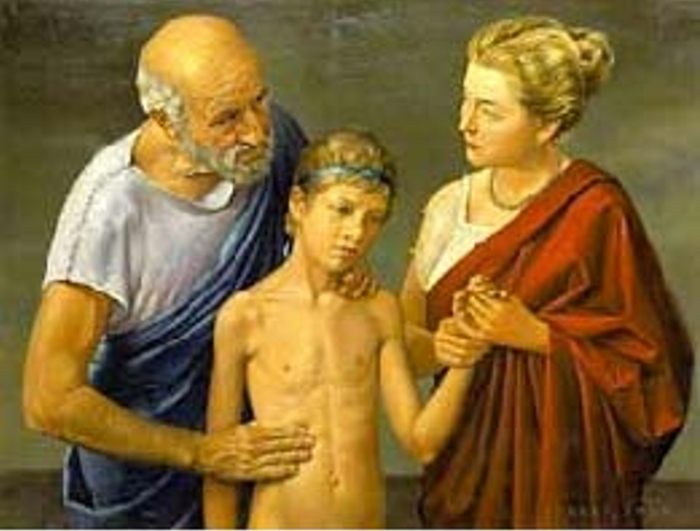
\includegraphics{images/005.jpg}
\caption{\textbf{ಚಿತ್ರ: \general{\enginline{18}} ಶ್ವಾಸೋಚ್ಚ್ವಾಸದ ಸಂಖ್ಯೆಯಲ್ಲಿ ಸ್ವಲ್ಪ ಇಳಿತಾಯ ಕಂಡುಬಂದು ಶ್ವಾಸ ಕಟ್ಟಿಕೊಳ್ಳುವ ಸಾಮರ್ಥ್ಯದಲ್ಲಿ ಹಾಗೂ ದೇಹಸಾಮರ್ಥ್ಯದಲ್ಲಿ ಹೆಚ್ಚಳ ತೋರಿಬಂತು.} }
\end{figure}

ಇವಲ್ಲದೆ ನರವ್ಯೂಹ ಮತ್ತು ನಿರ್ನಾಳ ಗ್ರಂಥಿಗಳ ಸಾಮರ್ಥ್ಯ, ರಕ್ತ, ಮಲ, ಮೂತ್ರ ಮೊದಲಾದುವುಗಳ ಸಮಗ್ರ ಪರೀಕ್ಷೆಗಳನ್ನು ವಿಸ್ತೃತವಾದ ರೀತಿಯಲ್ಲಿ, ವೈದ್ಯವಿಜ್ಞಾನ ಕ್ರಮದಲ್ಲಿ ನಡೆಸಲಾಯಿತು. ಇವನ್ನು ಯೋಗಾಭ್ಯಾಸಾರಂಭಕ್ಕೆ ಮೊದಲು ಹಾಗೂ ನಂತರ ಸಮರ್ಥ ವಿಜ್ಞಾನಿಗಳ ಮೂಲಕ ನಡೆಸಿ ಪರಿಶೀಲಿಸಲಾಯಿತು.

\textbf{ಇಂತಹ ವೈಜ್ಞಾನಿಕ ಅಧ್ಯಯನದ ಫಲಿತಾಂಶ}

ಯೋಗಾಭ್ಯಾಸ ನಡೆಸುತ್ತಿದ್ದವರ ದೇಹ ಮನಸ್ಸುಗಳಲ್ಲಾದ ಬದಲಾವಣೆಗಳು ನಿಜವಾಗಿಯೂ ಗಣನೀಯವಾಗಿದ್ದುವು. ಆ ಫಲಿತಾಂಶಗಳನ್ನು ತಿಳಿದುಕೊಳ್ಳಲು ಸಂತೋಷವೂ ಆಗಬಹುದು.

\begin{figure}
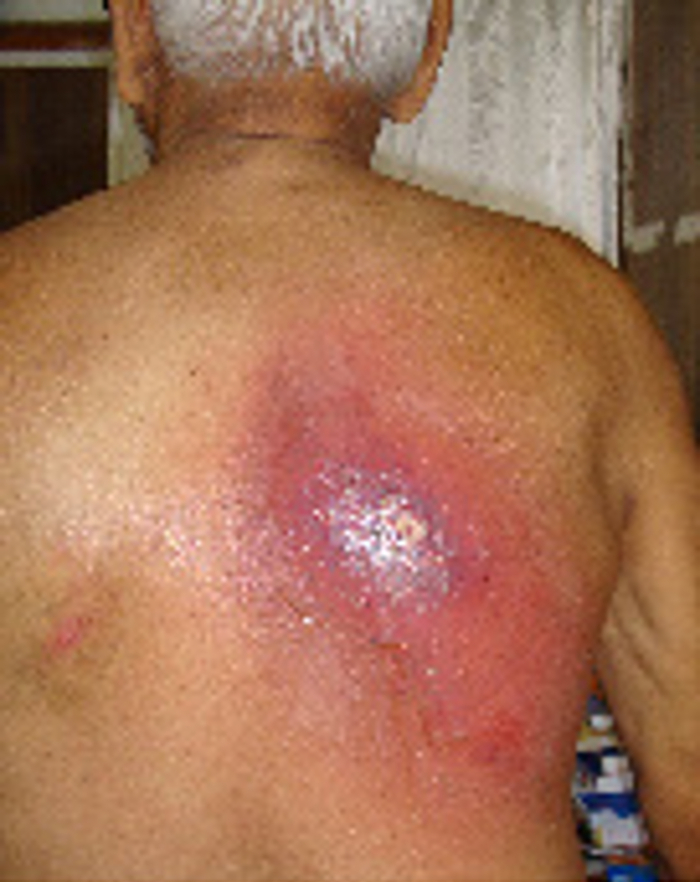
\includegraphics{images/006.jpg}
\caption{\textbf{ಚಿತ್ರ \general{\enginline{19}}:ಯೋಗಾಭ್ಯಾಸದಿಂದ ತೋರಿಬಂದ ಜೀವದ್ರವ್ಯ ಬದಲಾವಣೆಗಳ ಸುಧಾರಣ್} }
\end{figure}

ಹನ್ನೆರಡು ಪ್ರಮುಖ ಯೋಗಾಸನಗಳನ್ನು ಆರು ತಿಂಗಳ ಕಾಲ ಅಭ್ಯಾಸಗೈದ ಪರಿಣಾಮವಾಗಿ ದೇಹದ ತೂಕ ಕಡಿಮೆಯಾಯಿತು. ಹೊಟ್ಟೆಯ ಸುತ್ತಳತೆ ಕುಂದಿತು. ಶ್ವಾಸೋಚ್ಛ್ವಾಸದ ಸಂಖ್ಯೆ ಕಡಿಮೆಯಾಗಿ, ದೇಹಸಾಮರ್ಥ್ಯ ಹಾಗೂ ಶ್ವಾಸ ಕಟ್ಟಿಕೊಂಡಿರುವ ಸಮಯದ ಸಾಮರ್ಥ್ಯದಲ್ಲಿ ಹೆಚ್ಚಳ ತೋರಿ ಬಂತು. ಇ.ಇ.ಜಿ.ಯಲ್ಲಿ ಪ್ರಮುಖ ಅಲ್ಫಾ ತರಂಗಗಳು ತೋರಿಬರುವ ಉತ್ತಮ ಬದಲಾವಣೆ ಕಂಡುಬಂತು. ರಕ್ತದಲ್ಲಿ ದುಗ್ಧರಸದ ಕೊಲೆಸ್ಟರೋಲ್ \enginline{(Serum cholesterol)} ಮತ್ತು ಶರ್ಕರದ ಅಂಶ ಬಹುಮಟ್ಟಿಗೆ ಕಡಿಮೆಯಾದುವು. ದುಗ್ಧರಸದ ಪ್ರೊಟೀನ್ಸ್ \enginline{(Serum Proteins)} ಹೆಚ್ಚಾದುವು. \enginline{Plasma cortisol, Urinary corticoids including testosterone} ಗಳು ಹೆಚ್ಚಾದುದು ತೋರಿಬಂದರೆ \enginline{Plasma acetylcohlin} ಮತ್ತು \enginline{cholinestrase} ಮಟ್ಟ \enginline{(level)} ಕಡಿಮೆಯಾದುದನ್ನು ಕಾಣಲಾಯಿತು. ಜೀವದ್ರವ್ಯ ಪರಿಣಾಮ ದೃಷ್ಟಿಯಿಂದ ಯೋಗಾಭ್ಯಾಸದಿಂದಾಗಿ ರಕ್ತದ ಶರ್ಕರಾಂಶ ಮತ್ತು \enginline{cholesterol} ಕಡಿಮೆಯಾಯಿತು. \enginline{Serum Protein} ಹೆಚ್ಚಾಯಿತು.

\begin{center}
\enginline{\textbf{Neurohumoral changes after practice of yoga}}
\end{center}


\begin{figure}
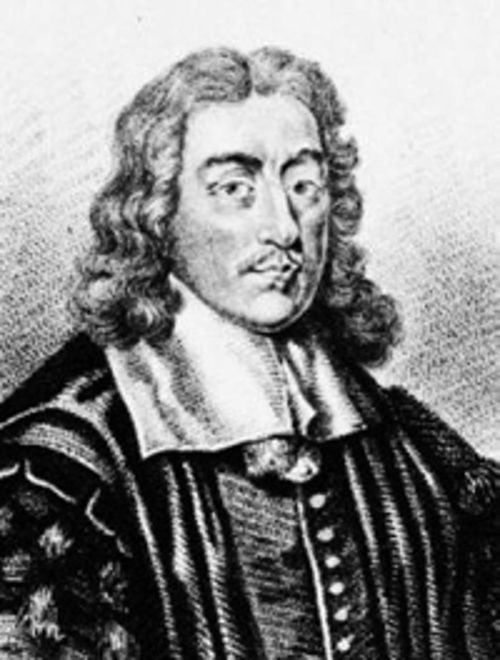
\includegraphics{images/007.jpg}
\caption{\textbf{ಚಿತ್ರ 20:ಯೋಗಾಭ್ಯಾಸದಿಂದುಂಟಾದ ನರರಾಸಾಯನಿಕ ಬದಲಾವಣೆಗಳು.} }
\end{figure}

\begin{center}
\enginline{\textbf{Urinary excretion of testosterone before and after six months of the practice of yoga.}}
\end{center}


\begin{figure}
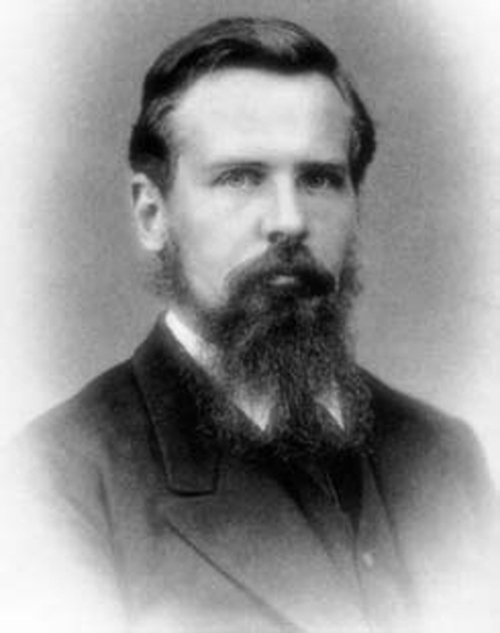
\includegraphics{images/008.jpg}
\caption{\textbf{ಚಿತ್ರ: \general{\enginline{21}} ಯೋಗಾಭ್ಯಾಸದ ಪರಿಣಾಮವಾಗಿ ಮೂತ್ರದಲ್ಲಿ ವಿಸರ್ಜಿಸಲ್ಪಡುವ ಹೆಚ್ಚಿನ \general{\enginline{Testosterone}} ಪ್ರಮಾಣ ಹೆಚ್ಚಿದ ಚೈತನ್ಯ ಹಾಗೂ ಕಾಮಸಾಮರ್ಥ್ಯವನ್ನು ಸೂಚಿಸುತ್ತದೆ.} }
\end{figure}

\begin{center}
\enginline{\textbf{Improved adrenocortical functions after YOGA practice.}}
\end{center}


\begin{figure}
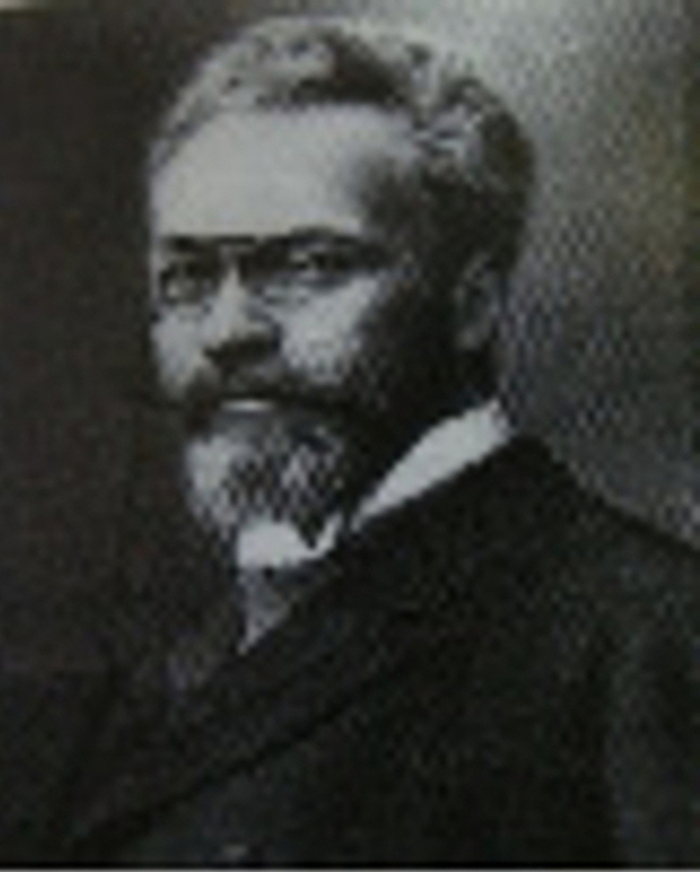
\includegraphics{images/009.jpg}
\caption{\textbf{ಚಿತ್ರ \general{\enginline{22}}: ಯೋಗಾಭ್ಯಾಸದ ಪರಿಣಾಮವಾಗಿ ಮೂತ್ರಜನಕಾಂಗಗಳ ಕಾರ್ಯನಿರ್ವಹಣೆಯಲ್ಲಿ ತೋರಿಬಂದ ಸುಧಾರಣೆ.} }
\end{figure}

\enginline{Acetycholine} ಮತ್ತು \enginline{Cholinesterase} ಮಟ್ಟ ಕಡಿಮೆಯಾಗಿ ಮಿದುಳಿನ ಕಾರ್ಯಾಚರಣೆಯಲ್ಲಿ ಶಾಂತ ಪರಿಸ್ಥಿತಿ ಉಂಟಾದುದು ತೋರಿಬಂತು.

ಯೋಗಾಭ್ಯಾಸದಿಂದಾಗಿ ಮೂತ್ರದಲ್ಲಿ \enginline{corticoids} ಮತ್ತು \enginline{catecholamine} ವಿಸರ್ಜನೆ ಹೆಚ್ಚಾದುದು ಕಂಡುಬಂತು.

ಸಮಗ್ರ ಯೋಗಾಭ್ಯಾಸವನ್ನು ನಡೆಸಿಕೊಂಡು ಬರುತ್ತಿರುವ ಸ್ವಯಂ ಸೇವಕರ ಮಾನಸಿಶಕ್ತಿಯ ಅಧ್ಯಯನವನ್ನೂ ಆರು ತಿಂಗಳ ನಂತರ ನಡೆಸಲಾಯಿತು. ಆಗ ನರದೌರ್ಬಲ್ಯ \enginline{(Neuroticism)} ಕಡಿಮೆಯಾಗಿ, ಮಾನಸಿಕ ಆಯಾಸದ ಮಟ್ಟ ಕುಗ್ಗಿದುದು ತೋರಿಬಂತು. ಮಾತ್ರವಲ್ಲದೆ \enginline{G.M.I Scores} ಸಹ ಬಹಳ ಕುಂದಿ ಬಂತು. ಬೌದ್ಧಿಕ ನಿರ್ವಹಣಾಶಕ್ತಿ ಮತ್ತು ಜ್ಞಾಪಕಶಕ್ತಿಯ ಹೆಚ್ಚಳ ಕಂಡು ಬಂತು. \enginline{(23, 24} ಮತ್ತು \enginline{25.)} ದೈಹಿಕ ಮಾನಸಿಕ ಸಂಕಟಗಳು ಕಡಿಮೆಯಾಗಿ ಆರೋಗ್ಯ ಸುಧಾರಣೆಗೊಂಡುದನ್ನು ಚಿತ್ರದಲ್ಲಿ ಕಾಣಬಹುದು.

ನರದೌರ್ಬಲ್ಯ ಹಾಗೂ ಮಾನಸಿಕ ಆಯಾಸ ಕುಂದಿಬರುವುದನ್ನೂ ಕಾಣಬಹುದು.

\textbf{ಆಯ್ದು ಕೆಲವು ಯೋಗಾಸನ ಅಭ್ಯಾಸದ ಪರಿಣಾಮ}

ಆಯ್ದ ಕೆಲ ಯೋಗಾಸನಗಳ, ಮುಖ್ಯವಾಗಿ—ಶೀರ್ಷಾಸನ, ಸರ್ವಾಂಗಾಸನ, ಹಲಾಸನ ಇವುಗಳ ಪರಿಣಾಮವನ್ನು ಕಂಡುಹಿಡಿಯಲು ಪ್ರತ್ಯೇಕ ಅಧ್ಯಯನ ಕೈಗೊಳ್ಳಲಾಯಿತು. ಇದರ ಉದ್ದೇಶ, ಪ್ರಮುಖ ಆಸನಗಳನ್ನು ಮಾತ್ರ ಅಭ್ಯಾಸ ಗೈಯುವುದರಿಂದ ತಕ್ಕ ಪ್ರಯೋಜನ ದೊರಕಬಹುದೇ—ಎಂಬುದನ್ನು ತಿಳಿದು ಕೊಳ್ಳುವುದಾಗಿದೆ.

ಶಾರೀರಿಕ ಮತ್ತು ಜೀವರಾಸಾಯನಿಕ ಸುಧಾರಣೆಯ ವಿಚಾರದಲ್ಲಿ ಮೇಲೆ ಹೇಳಿದ್ದ ಸಮಗ್ರ ಆಸನಗಳ ಅಭ್ಯಾಸದ ಪರಿಣಾಮಕ್ಕೂ, ಈ ನಿರ್ದಿಷ್ಟ ಆಸನಗಳ ಪರಿಣಾಮಕ್ಕೂ ಹೆಚ್ಚಿನ ವ್ಯತ್ಯಾಸ ಕಂಡುಬರಲಿಲ್ಲ. ಆದರೆ ಸರ್ವಾಂಗಾಸನದ ಅಭ್ಯಾಸದಿಂದ ದೈಹಿಕ ಮತ್ತು ನಿರ್ನಾಳ ಗ್ರಂಥಿಗಳ \enginline{(Endocrines)} ಸುಧಾರಣೆ ವಿಶಿಷ್ಟ ರೀತಿಯಲ್ಲಿ ತೋರಿಬಂತು. ಅದಕ್ಕೆ ಕಾರಣ ಮೂತ್ರ ಜನಕಾಂಗ ಹಾಗೂ ಥೈರೋಡ್ ಚಟುವಟಿಕೆಗಳಲ್ಲಿ ಹೆಚ್ಚಿನ ಸುಧಾರಣೆ ತೋರಿಬಂದಿರುವುದಾಗಿರಬೇಕು. ಶೀರ್ಷಾಸನದಿಂದಲೂ ಈ ಪರಿಣಾಮ ಒದಗಿಬಂದಿದ್ದರೂ ಇಷ್ಟು ಗಮನಾರ್ಹ ಸುಧಾರಣೆ ತೋರಿಬಂದಿಲ್ಲ. ಹಲಾಸನದಿಂದ ತೋರಿಬಂದ ಬದಲಾವಣೆ ಬಹು ಕಡಿಮೆ.

\begin{center}
\enginline{\textbf{Improved health pattern after practice of yoga}}
\end{center}


\begin{figure}
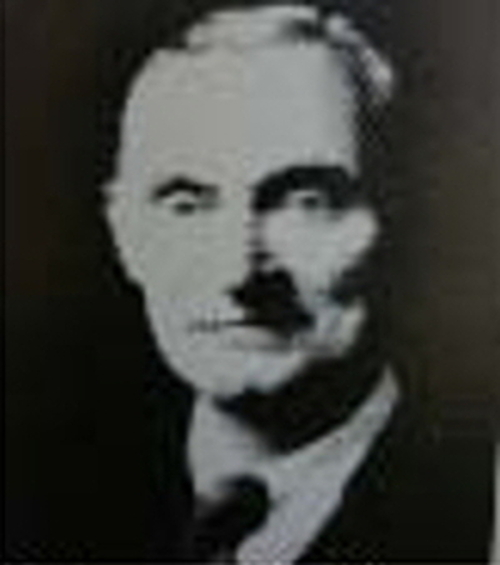
\includegraphics{images/010.jpg}
\caption{ಚಿತ್ರ \enginline{23}: ಯೋಗಾಭ್ಯಾಸದಿಂದಾಗಿ ಸುಧಾರಿತ ದೈಹಿಕ ಮಾನಸಿಕ ಆರೋಗ್ಯ.}
\end{figure}

ಬೇರೆಬೇರೆ ಯೋಗಾಸನಗಳನ್ನು ಪ್ರತ್ಯೇಕವಾಗಿ ಅಥವಾ ಇತರ ನಿರ್ದಿಷ್ಟ ಯೋಗಾಸನಗಳೊಡನೆ ನಡೆಸಿಕೊಂಡು ಬಂದುದರ ಪರಿಣಾಮವನ್ನೂ ಪರಿಶೀಲಿಸ ಲಾಯಿತು. ಅದರಿಂದ ಒದಗಿಬರುವ ಜೈವಿಕ ಪ್ರತಿಕ್ರಿಯೆಗಳ ವಿಚಾರದಲ್ಲಿ ಇನ್ನಷ್ಟು ಅಧ್ಯಯನಗೈದಾಗ, ದೇಹದ ಯಾವ ಯಾವ ಅವಯವಗಳ ಮೇಲೆ ಎಂತೆಂತಹ ಪರಿಣಾಮ ತೋರಿಬರುತ್ತದೆಂಬುದೂ ತಿಳಿದು ಬಂತು. ಈ ವಿಚಾರವನ್ನು ಮತ್ತಷ್ಟು ಆಳವಾಗಿ ಅಧ್ಯಯನ ಮಾಡಿದರೆ ಇಂತಿಂತಹ ಶರೀರದ ನ್ಯೂನತೆಗೆ ಇಂತಿಂತಹ ಯೋಗಾಭ್ಯಾಸ ಮಾಡಬೇಕು; ಅಥವಾ ಇಂತಹ ಕಾಯಿಲೆ ನಿವಾರಣೆಗೆ ಈ ತರದ ಯೋಗಾಭ್ಯಾಸ ನಡೆಸಬೇಕು; ಎಂದು ಮೊದಲಾಗಿ ಹೇಳಲೂ ಸಾಧ್ಯವಾಗಬಹುದು. ಬೇರೆಬೇರೆ ತರದ ಜನರ ವಿವಿಧ ಕೊರತೆಗಳಿಗೊಪ್ಪುವ ಯೋಗಾಸನಗಳನ್ನು ಔಷಧಿ ಯಂತೆ ಹೇಳಿಕೊಡಲಾಗಬಹುದು. ಅಥವಾ ತಕ್ಕ ಔಷಧಿಯೊಂದಿಗೆ ಯೋಗೋಪ ಚಾರವನ್ನು ಹೇಳಿಕೊಟ್ಟು ಅವರನ್ನು ಸಂಪೂರ್ಣ ಸ್ವಸ್ಥರನ್ನಾಗಿಸಲೂಬಹುದು.

\begin{figure}
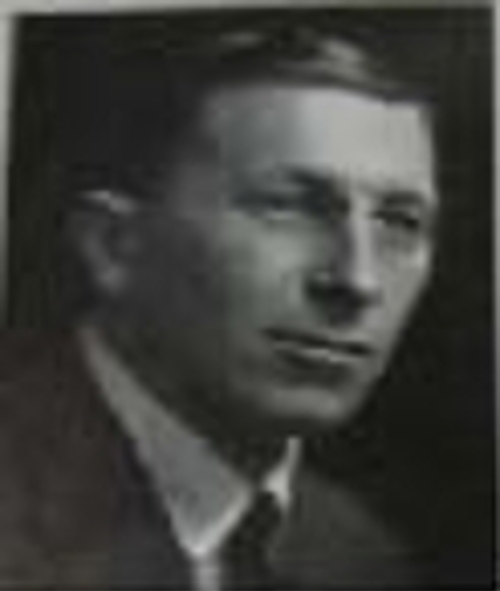
\includegraphics{images/011.jpg}
\caption{\textbf{ಚಿತ್ರ \general{\enginline{24:}} ಯೋಗಾಭ್ಯಾಸದಿಂದ ತೋರಿಬಂದ ವೈಯಕ್ತಿಕ ಸಾಧನೆ.} }
\end{figure}

\textbf{ಪ್ರಾಣಾಯಾಮದ ಅಭ್ಯಾಸ:} ಆರೋಗ್ಯವಂತ ವ್ಯಕ್ತಿಗಳ ತಂಡ ಒಂದನ್ನು ಆಯ್ಕೆಗೈದು ಅವರು 'ಉಜ್ವೈ' ಮತ್ತು 'ಭಸ್ತ್ರಿಕಾ' ವಿಧಾನದ ಪ್ರಾಣಾಯಾಮಾಭ್ಯಾಸ ವನ್ನು ಆರು ತಿಂಗಳಕಾಲ ತಕ್ಕ ರೀತಿಯಲ್ಲಿ ನಡೆಸುವ ವ್ಯವಸ್ಥೆ ಮಾಡಲಾಯಿತು. ಆಮೇಲೆ ಅವರ ಶ್ವಾಸಕೋಶ ಮತ್ತು ಹೃದಯದ ಚಟವಟಿಕೆಗಳನ್ನು ಪರೀಕ್ಷಿಸಿ ನೋಡಿದಾಗ ಅವರೆಲ್ಲರಲ್ಲಿಯೂ ಗಣನೀಯ ಸುಧಾರಣೆ ಕಂಡು ಬಂತು. ಹಾಗೆಯೇ ಮೂತ್ರಜನಕಾಂಗಗಳ \enginline{(Adernocortical function)} ಚಟುವಟಿಕೆಗಳಲ್ಲೂ ಸುಧಾರಣೆ ತೋರಿಬಂತು.

\textbf{ಧ್ಯಾನದ ಅಭ್ಯಾಸ:} ಇದಕ್ಕಾಗಿ ಭಾರತೀಯ ಹಾಗೂ ಪಾಶ್ಚಾತ್ಯ ದೇಶಗಳ ಸ್ವಯಂಸೇವಕರ ತಂಡಗಳೆರಡನ್ನು ಆಯ್ದುಕೊಳ್ಳಲಾಯಿತು. ಇವರು ವಿಪಾಸನಾ ರೀತಿಯ ಧ್ಯಾನಾಭ್ಯಾಸವನ್ನು ಹತ್ತುದಿನಗಳವರೆಗೆ ನಡೆಸಿಕೊಂಡು ಬರುವಂತೆ ಪ್ರತ್ಯೇಕ ಧ್ಯಾನಶಿಬಿರದಲ್ಲಿ ವ್ಯವಸ್ಥೆಗೈಯಲಾಯಿತು.

ಧ್ಯಾನಾಭ್ಯಾಸಕ್ಕೆ ಮೊದಲು ಮತ್ತು ನಂತರ ಅವರ ಮಾನಸಿಕ ಹಾಗೂ ದೈಹಿಕ ಪರಿಸ್ಥಿತಿಯ ಅಧ್ಯಯನ ನಡೆಸಲಾಯಿತು. ಹತ್ತು ದಿನಗಳ ಧ್ಯಾನಾಭ್ಯಾಸದ ನಂತರ ಅವರ \enginline{Level of Plasma Cortisol} ಮತ್ತು \enginline{Urinary Nitrogen ಗಣನೀಯ ಪ್ರಮಾಣದಲ್ಲಿ ಕಡಿಮೆಯಾದುದು ತೋರಿಬಂತು. ಹಾಗೆಯೇ ರಕ್ತದಲ್ಲಿ \general{\enginline{R.B.C.}} \general{\enginline{Acetycholine, R.B.C. Cholinesterase, Plasma Catecholamins}} ಮತ್ತು \general{\enginline{Plasma Histaminase}} ಮುಂತಾದ ಬೇರೆಬೇರೆ \general{\enginline{Neurohumors}} ಗಳಲ್ಲಿ ಗಣನೀಯ ಪ್ರಮಾಣದ ಹೆಚ್ಚಳ ತೋರಿಬಂತು. ಈ ಧ್ಯಾನಾಭ್ಯಾಸಗೈದವರು ದೈಹಿಕವಾಗಿ ಶಾಂತಿ ಸಮಾಧಾನದಿಂದಿದ್ದರು. ಆದರೂ ಮಾನಸಿಕವಾಗಿ ಹೆಚ್ಚು ಕ್ರಿಯಾಶೀಲರೂ ಚುರುಕಾದವರೂ ಆಗಿ ತೋರಿಬಂದರು.}

\begin{figure}
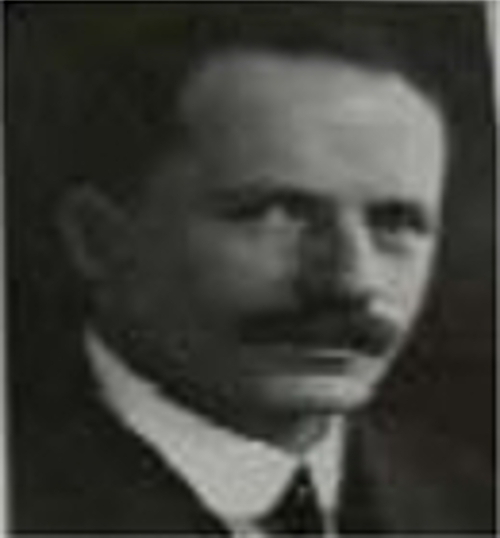
\includegraphics{images/012.jpg}
\caption{\textbf{ಚಿತ್ರ \general{\enginline{25}}: ಯೋಗಾಭ್ಯಾಸದ ಪರಿಣಾಮವಾಗಿ ನಿರ್ವಹಣಾಶಕ್ತಿ, ಜ್ಞಾಪಕಶಕ್ತಿಗಳು ಸುಧಾರಣೆಗೊಂಡುದನ್ನು ಕಾಣಬಹುದು.} }
\end{figure}

ಬೇರೆಬೇರೆ ತರದ ಧ್ಯಾನಾಭ್ಯಾಸಗಳು ಮನಸ್ಸಿನ ಏಕಾಗ್ರತಾಶಕ್ತಿಯನ್ನು ಹೆಚ್ಚಿಸುತ್ತವೆ. ಉದ್ವೇಗಕರ ಭಾವನೆಗಳನ್ನು ಕಡಿಮೆಗೈಯುತ್ತವೆ. ಅದರಲ್ಲಿಯೂ ಬುದ್ಧಧರ್ಮದಲ್ಲಿ ಹೇಳಲಾದ ವಿಪಾಸನಾಧ್ಯಾನವು ಮನಶ್ಯಕ್ತಿ ಮತ್ತು ಮನಶ್ಯಾಂತಿ ಯನ್ನು ಹೆಚ್ಚಿಸುವಲ್ಲಿ ತುಂಬಾ ಪ್ರಭಾವಶಾಲಿಯಾಗಿದೆ. ಇಂದಿನ ನಾನಾತರದ ಮಾನಸಿಕ ಒತ್ತಡ ತುಂಬಿದ ವಾತಾವರಣದಲ್ಲಿ ಮಾನವನಿಗೆ ಈ ತರದ ಪ್ರಾರ್ಥನಾಮಯ ಧ್ಯಾನವು ಸಮಯೋಚಿತವಾಗಿದೆ.

\begin{center}
\enginline{\textbf{Some physiological and biochemical changes after 3 months of the practice of Pranayam}}
\end{center}


\begin{figure}
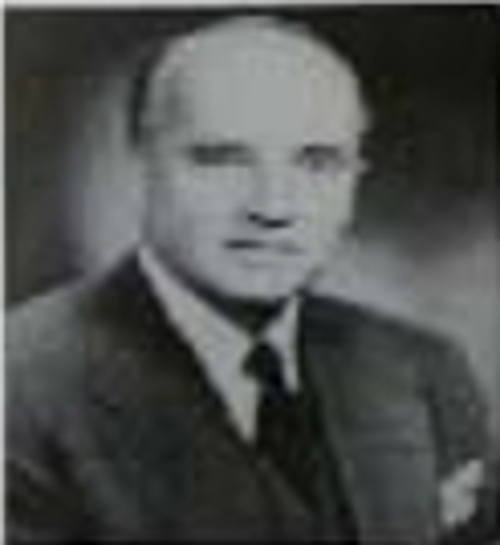
\includegraphics{images/013.jpg}
\caption{ಚಿತ್ರ \enginline{26}: ಮೂರು ತಿಂಗಳ ಪ್ರಾಣಾಯಾಮಾಭ್ಯಾಸದ ನಂತರ ತೋರಿಬಂದ ಶಾರೀರಿಕ ಮತ್ತು ಜೀವರಾಸಾಯನಿಕ ಬದಲಾವಣೆಗಳು.}
\end{figure}

ಧ್ಯಾನವು ಅಷ್ಟಾಂಗ ಯೋಗಗಳ ಪ್ರಮುಖ ಅಂಗವಾಗಿದೆ. ಈ ಧ್ಯಾನ ಮಾನವದೇಹದೊಳಗೆ ಉಂಟುಮಾಡುವ ಜೀವರಾಸಾಯನಿಕ ಪರಿಣಾಮ ಏನೆಂಬ ವಿಚಾರದಲ್ಲಿ ನಾವು ಅಧ್ಯಯನ ನಡೆಸಬಯಸಿದೆವು. ಅದೃಷ್ಟವಶಾತ್ ವಾರಾಣಸಿಯ ಬುದ್ಧವಿಹಾರದಲ್ಲಿ \enginline{1973} ಡಿಸೆಂಬರ್ \enginline{1974} ಜನವರಿ ತಿಂಗಳುಗಳಲ್ಲಿ ವಿಪಾಸನಾ ಯೋಗ ಶಿಬಿರವನ್ನು ಏರ್ಪಡಿಸಲಾಗಿತ್ತು. ಅಲ್ಲಿ ಧ್ಯಾನಾಭ್ಯಾಸಗೈಯಲು ಬಂದ ಅಭ್ಯರ್ಥಿಗಳ ದೇಹದೊಳಗಿನ ಜೀವರಾಸಾಯನಿಕ ಬದಲಾವಣೆಗಳನ್ನು ಅಧ್ಯಯನ ಮಾಡಲು, ಒದಗಿಬಂದ ಅವಕಾಶವನ್ನು ಸದುಪಯೋಗ ಮಾಡಿಕೊಂಡೆವು.

ಈ ಅಧ್ಯಯನದಲ್ಲಿ ಇನ್ನೊಂದು ಕುತೂಹಲಕಾರೀ ವಿಚಾರವೂ ಇತ್ತು. ಅದೇನೆಂದರೆ ಅಲ್ಲಿ ಇಂಗ್ಲಿಷ್ ಮಾಧ್ಯಮದ ಪಾಶ್ಚಾತ್ಯ ದೇಶಗಳ ಧ್ಯಾನಾಭ್ಯಾಸಿಗಳ ಹತ್ತು ಜನರ ತಂಡ ಒಂದು; ಹಿಂದೀ ಮಾಧ್ಯಮದ ಹತ್ತು ಭಾರತೀಯ ಧ್ಯಾನಾಭ್ಯಾಸಿಗಳ ತಂಡ ಇನ್ನೊಂದು. ಇವರಿಗೆ ಬೇರೆಬೇರೆ ಶಿಬಿರಗಳನ್ನೇರ್ಪಡಿಸ ಲಾಗಿತ್ತು. ಪಾಶ್ಚಾತ್ಯ ದೇಶದ ಬಿಳಿಯರ ಹಾಗೂ ಭಾರತೀಯ ಸ್ವಯಂಸೇವಕರ ಜೀವರಾಸಾಯನಿಕ ಪರಿಣಾಮಗಳು ಧ್ಯಾನಾಭ್ಯಾಸದಿಂದ ಏನೆಲ್ಲ ಬದಲಾವಣೆ ಗೊಳ್ಳುತ್ತವೆ ಎಂದು ಹೋಲಿಸಿ ನೋಡಲಿಕ್ಕೂ ನಮಗೆ ಅನುಕೂಲವಾಯಿತು. ಈ ಎರಡು ಶಿಬಿರಗಳಿಂದಲೂ ಹತ್ತುಹತ್ತರಂತೆ ಸ್ವಯಂಸೇವಕರನ್ನಾಯ್ಕೆ ಮಾಡಿಕೊಂಡು ನಮ್ಮ ಅಧ್ಯಯನವನ್ನು ನಾವು ನಡೆಸಿಕೊಂಡು ಬಂದೆವು.

ಆ ಸ್ವಯಂಸೇವಕರು ಶಿಬಿರದೊಳಗೆಯೇ ನಿಯಮಬುದ್ಧ ಜೀವನ ನಡೆಸಿ ಕೊಂಡು ಸಸ್ಯಾಹಾರಿಗಳಾಗಿ ಇರಬೇಕಾಗಿತ್ತು. ಯಾವುದೇ ತರದ ಮಾದಕ ವಸ್ತುಗಳ ಸೇವನೆ ನಿಷಿದ್ಧವಾಗಿತ್ತು. ಧ್ಯಾನಶಿಬಿರ ಮುಗಿಯುವವರೆಗೆ ಅವರನ್ನು ಹೊರ ಹೋಗಬಿಡುತ್ತಿರಲಿಲ್ಲ. ಮೊದಲ ಮೂರು ದಿನಗಳಲ್ಲಿ ಪ್ರಾಣಾಯಾಮ ಮತ್ತು ಧಾರಣಾವಿಧಾನಗಳನ್ನು ಕಲಿಸಿ, ಮನಸ್ಸಿನ ಏಕಾಗ್ರತೆ ಸಾಧಿಸಲಿಕ್ಕೆ ಅವರಿಗೆ ಕಲಿಸಿಕೊಡಲಾಯಿತು. ನಂತರ ಅವರು ಸಂಪೂರ್ಣ ಅಂತರ್ಮುಖಿಗಳಾಗಿ ಧ್ಯಾನಾ ಭ್ಯಾಸಗೈಯಲು ಹೇಳಿಕೊಡಲಾಯಿತು. ಇಂತಹ ವಿಪಾಸನಾ ರೂಪದ ಧ್ಯಾನಾಭ್ಯಾಸವನ್ನು ಅವರೆಲ್ಲ ದಿನಕ್ಕೆ \enginline{8–10} ಘಂಟೆಗಳ ಕಾಲ ಎಡೆಬಿಡದೆ ಹತ್ತು ದಿನಗಳವರೆಗೆ ನಡೆಸಿಕೊಂಡು ಬಂದರು.

ಅದೂ ಅಲ್ಲದೆ, ಈ ಧ್ಯಾನಾಭ್ಯಾಸದ ಸಾಕಷ್ಟು ಅನುಭವವಿದ್ದ ಭಾರತೀಯ ಸ್ವಯಂಸೇವಕನೊಬ್ಬ, ಧ್ಯಾನಮಗ್ನನಾಗಿದ್ದಾಗ ಆತನ ರಕ್ತ ಪರೀಕ್ಷೆಯನ್ನು ನಡೆಸಲಾಯಿತು. ಆತನ ದೇಹದಿಂದ ಮೊದಲೇ ವ್ಯವಸ್ಥೆಗೊಳಿಸಲಾಗಿದ್ದ ರೀತಿಯಲ್ಲಿ \enginline{Serial Blood Samples} ತೆಗೆದುಕೊಳ್ಳಲಾಯಿತು. ಮಾತ್ರವಲ್ಲದೆ ಧ್ಯಾನಾ ಭ್ಯಾಸಕ್ಕೆ ಮೊದಲು, ಧ್ಯಾನಕಾಲದಲ್ಲಿ ಮತ್ತು ಧ್ಯಾನ ಮುಗಿದು \enginline{45} ನಿಮಿಷಗಳ ನಂತರ, \enginline{EEG., EOG., EMG} ಮತ್ತು \enginline{EKG records} ಗಳನ್ನು ಸಂಗ್ರಹಿಸಿ ಅವನ್ನೆಲ್ಲ ಪರಿಶೀಲಿಸಲಾಯಿತು.

\begin{figure}
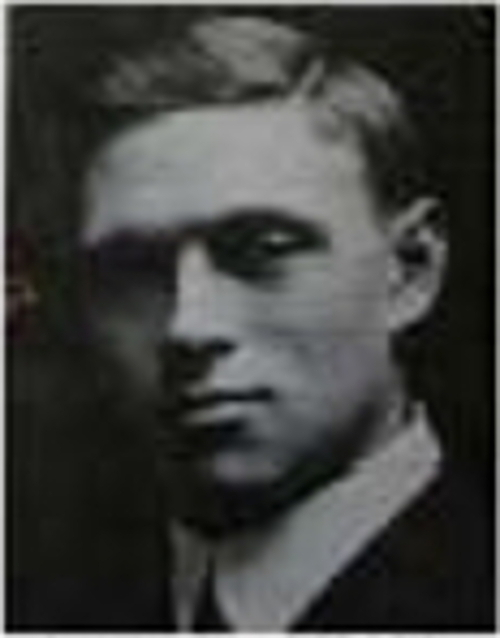
\includegraphics{images/014.jpg}
\end{figure}

ಧ್ಯಾನಾಭ್ಯಾಸ ಮುಗಿದು ಹನ್ನೊಂದನೇ ದಿನ ಸ್ವಯಂಸೇವಕರನ್ನು ಪರೀಕ್ಷಿಸಿ ನೋಡಿದಾಗ ಅವರ ರಕ್ತದಲ್ಲಿ ಮೊದಲಿಗಿಂತ ಬಹುಹೆಚ್ಚಿನ ಬದಲಾವಣೆ ತೋರಿಬಂತು. ರಕ್ತದ \enginline{Acetylcholine, Cholinesterase, Histaminase} ಮತ್ತು \enginline{Catecholamine} ಮಟ್ಟದಲ್ಲಿ. ಧ್ಯಾನಾಭ್ಯಾಸಕ್ಕೆ ಮೊದಲು ಇದ್ದ ಮಟ್ಟ ಕ್ಕಿಂತ ಸ್ಪಷ್ಟವಾದ ಹೆಚ್ಚಳ ತೋರಿಬಂತು. ಇದು ಎರಡೂ ಶಿಬಿರಗಳ ಸ್ವಯಂ ಸೇವಕರಲ್ಲೂ ಕಂಡುಬಂದುವು. \enginline{Plasma Cortisol, Urinary Corticoids} ಮತ್ತು \enginline{Nitrogen} ಗಳು ಕಡಿಮೆಯಾದುದು ಕಂಡುಬಂತು. ಇವನ್ನೆಲ್ಲ ಕೆಳಗಿನ ಕೋಷ್ಟಕಗಳಲ್ಲಿ ಕಾಣಬಹುದು.

ಮೇಲೆ ಹೇಳಿದ ಧ್ಯಾನಾಭ್ಯಾಸದಿಂದಾದ ಬದಲಾವಣೆಗಳನ್ನು ವಿಶ್ಲೇಷಿಸಿದಾಗ ಭಾರತೀಯ ಶಿಬಿರಸ್ಥರಕ್ಕಿಂತ ಪಾಶ್ಚಾತ್ಯರ ಶಿಬಿರಸ್ಥರಲ್ಲಿ ಆ ಸುಧಾರಣೆ ಹೆಚ್ಚಾಗಿ ಮತ್ತು ಸ್ಪಷ್ಟವಾಗಿ ಕಂಡುಬಂತು. \enginline{Urinary Nitrogen} ಗಣನೀಯ ಪ್ರಮಾಣ ದಲ್ಲಿ ಕುಂದಿಬಂದುದು ಪಾಶ್ಚಾತ್ಯರ ಯೋಗಶಿಬಿರಸ್ಥರಲ್ಲಿ ತೋರಿಬಂದ ಮಟ್ಟಕ್ಕೆ ಭಾರತೀಯ ಧ್ಯಾನಾಭ್ಯಾಸಿಗಳಲ್ಲಿ ಕಂಡುಬರಲಿಲ್ಲ.

ಸಂಪೂರ್ಣ ತರಬೇತಿ ಪಡೆದ ಆಯ್ದ ಸ್ವಯಂಸೇವಕನೊಬ್ಬನು ಧ್ಯಾನಾಸಕ್ತ ನಾಗಿರುವಾಗ ತೆಗೆದ ರಕ್ತವನ್ನು ಕ್ರಮಪ್ರಕಾರ ಪರೀಕ್ಷಿಸಿದಾಗ \enginline{Acetylcholine} ಮತ್ತು \enginline{Cholinesterase} ಮಟ್ಟದಲ್ಲಿ ಹೆಚ್ಚಳ ತೋರಿಬಂತು. ಆದರೆ \enginline{Catecholamine} ಮತ್ತು \enginline{Histamines} ಗಳಲ್ಲಿ ಗಣನೀಯ ಬದಲಾವಣೆಗಳು ತೋರಿಬರಲಿಲ್ಲ. ಧ್ಯಾನಾಭ್ಯಾಸ ಕಾಲದಲ್ಲಿ \enginline{EEG records} ಪರಿಶೀಲಿಸಿದಾಗ \enginline{Neurohumoral} ಬದಲಾವಣೆಗನುಗುಣವಾದ ವ್ಯತ್ಯಾಸಗಳು ತೋರಿಬಂದುವು.

ಈ ಮೊದಲೇ ಹೇಳಿದ್ದಂತೆ ವಿಪಾಸನಾಧ್ಯಾನವೆಂಬುದು ಬುದ್ಧ ಧರ್ಮದಲ್ಲಿ ಹೇಳಲಾದ ಧ್ಯಾನಕ್ರಮವಾದ್ದರಿಂದ ಅದು ಮನಸ್ಸಿನ ಅವಧಾನದ ಹೆಚ್ಚಳ ಉಂಟು ಮಾಡುತ್ತದೆ. ಧ್ಯಾನಾಭ್ಯಾಸಕಾಲದಲ್ಲಿ ತನ್ನ ಮನಸ್ಸನ್ನು ಯೋಗಿಯು ಒಂದೇ ವಿಷಯದ ಮೇಲೆ ಕೇಂದ್ರೀಕರಿಸಿಕೊಂಡಿರುತ್ತಾನೆ. ಹಾಗಾಗಿ ಆತ ಮಾನಸಿಕವಾಗಿ ಬಹಳ ಎಚ್ಚರಿಕೆಯಿಂದಿರುತ್ತಾನೆ. ದೈಹಿಕವಾಗಿ ನೋಡುವಾಗ ಪ್ರಶಾಂತಚಿತ್ತನಾಗಿ ತೋರಿದರೂ ಮಾನಸಿಕವಾಗಿ ಬಹು ಚುರುಕಾಗಿಯೂ ಎಚ್ಚರವಾಗಿಯೂ ಇರುತ್ತಾನೆ.

ನಾವು ಮಾಡಿದ ಅಧ್ಯಯನದಿಂದಲೂ ಈ ಅಂಶ ಸ್ಪಷ್ಟವಾಗಿ ಕಂಡುಬಂದಿದೆ. ಧ್ಯಾನದಿಂದಾಗಿ \enginline{Plasma Cortisol, Urinary Nitrogen and Corticoids} ಮುಂತಾದುವು ಇಳಿದಿರುವ ಕಾರಣ ಮಾನಸಿಕ ಒತ್ತಡ ಕಡಿಮೆಯಾಗಿದೆ ಎಂದು ತಿಳಿದುಬರುತ್ತದೆ. ಆದರೆ ರಕ್ತದಲ್ಲಿ \enginline{Neurohumoral Activity} ಹೆಚ್ಚಿಬಂದು, ಅದಕ್ಕನುಗುಣವಾದ \enginline{EEG} ಯಲ್ಲಿ ತೋರಿಬರುವ ಬದಲಾವಣೆ ಮಾನಸಿಕವಾಗಿ ಬಹಳ ಎಚ್ಚರಗೊಂಡವನಾಗಿಯೂ, ಚುರುಕಾಗಿಯೂ ಆತ ಇದ್ದಾನೆಂಬುದನ್ನು ಸೂಚಿಸುತ್ತದೆ.

\begin{center}
\enginline{\textbf{Endocrine and metabolic changes after a course of meditation}}
\end{center}


\begin{figure}
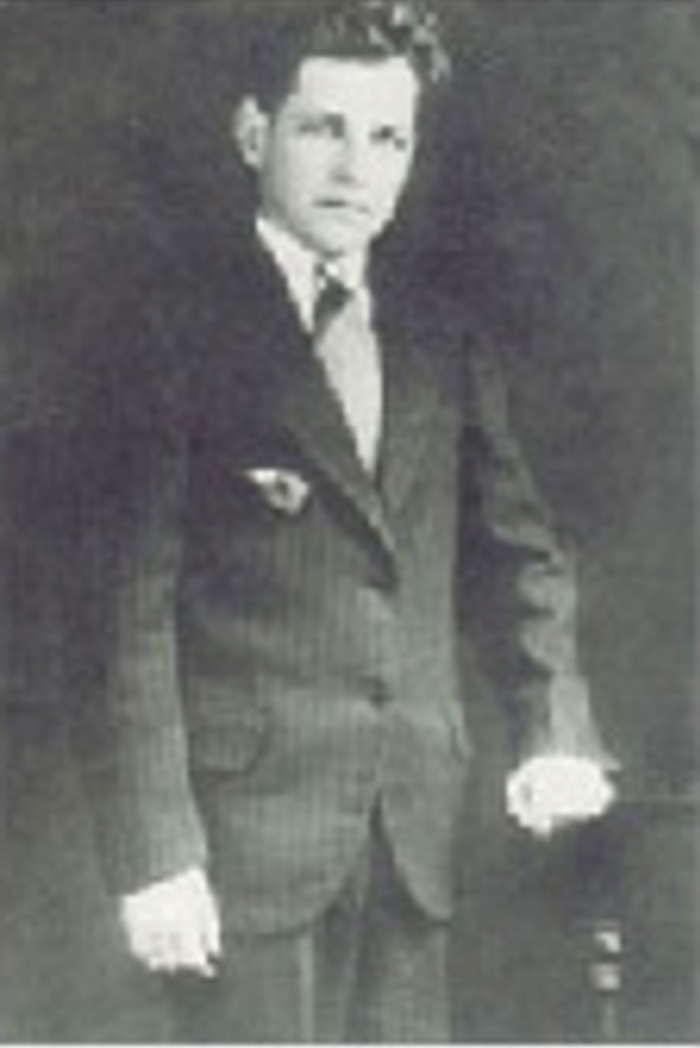
\includegraphics{images/015.jpg}
\caption{ಚಿತ್ರ \enginline{28:} ಧ್ಯಾನಾಭ್ಯಾಸದ ನಂತರ ತೋರಿಬಂದ ಬದಲಾವಣೆಗಳು}
\end{figure}

ಹೀಗೆ ಮೇಲೆ ಹೇಳಿದ ಧ್ಯಾನಾಭ್ಯಾಸದಿಂದ ಮಾನಸಿಕ ಒತ್ತಡದ ಮಟ್ಟ ಕಡಿಮೆಯಾಗುತ್ತದೆ. ಅದರಿಂದಾಗಿ ದೇಹದಲ್ಲಿ ಜೀವದ್ರವ್ಯ ಬದಲಾವಣೆಯ ವೇಗ ಕುಂದುತ್ತದೆ. ಅಷ್ಟೇ ಅಲ್ಲದೆ ಅಂತಹ ಧ್ಯಾನಭ್ಯಾಸಿಯು ಮಾನಸಿಕವಾಗಿ ಚುರುಕು ಯೋಗ ಗೊಂಡು, ಒಂದು ನಿರ್ದಿಷ್ಟ ವಿಷಯದಲ್ಲಿ ತನ್ನ ಮನಸ್ಸನ್ನು ಕೇಂದ್ರೀಕರಿಸಲೂ ಸಮರ್ಥನಾಗುತ್ತಾನೆ. ಈ ಮೊದಲಾದ ಅಂಶ ಆತನ ದೇಹದ ಜೀವರಾಸಾಯನಿಕ ಬದಲಾವಣೆಯ ಅಧ್ಯಯನದಿಂದ ತಿಳಿದುಬರುತ್ತದೆ.

\begin{center}
\enginline{\textbf{Neurohumoral changes during and immediately after meditation}}
\end{center}


\begin{figure}
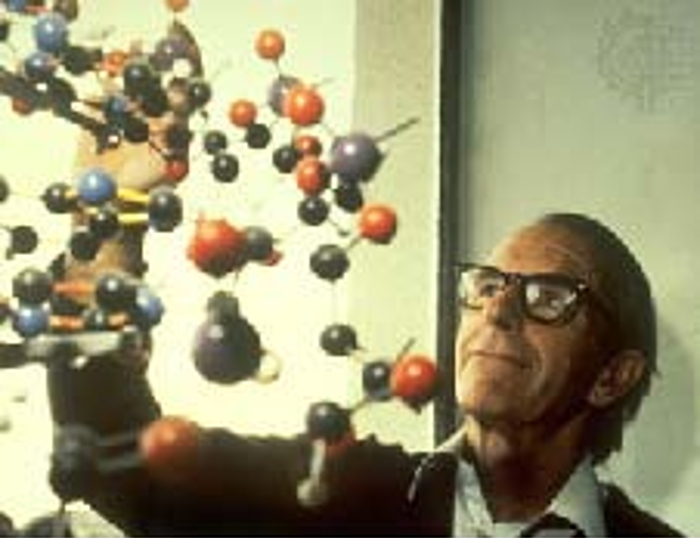
\includegraphics{images/016.jpg}
\caption{ಚಿತ್ರ \enginline{29:} ಧ್ಯಾನಾಭ್ಯಾಸಕಾಲದಲ್ಲಿ \enginline{acetycholine} ಮಟ್ಟವು ರಕ್ತದಲ್ಲಿ ಗಣನೀಯ ಪ್ರಮಾಣದಲ್ಲಿ ಹೆಚ್ಚಿ ಉಳಿದ ಬದಲಾವಣೆಗಳು ವಿಶೇಷವಾಗಿ ಹೆಚ್ಚದೆ ಇರುವುದನ್ನು ಕಾಣಬಹುದಾಗಿದೆ.}
\end{figure}

\textbf{ಆಸನ, ಪ್ರಾಣಾಯಾಮ ಮತ್ತು ವಿಶ್ರಾಂತಿ–ಇವುಗಳ ಸಂಯುಕ್ತ ಅಭ್ಯಾಸ}

ಆಸನ, ಪ್ರಾಣಾಯಾಮ ಮತ್ತು ಧ್ಯಾನಗಳ ಪರಿಣಾಮವಿಚಾರದಲ್ಲಿ ಪ್ರತ್ಯೇಕ ಪ್ರತ್ಯೇಕವಾದ ಅಧ್ಯಯನಗಳನ್ನು ನಡೆಸಿದ ನಂತರ, ಈ ಮೂರು ಯೋಗಾಭ್ಯಾಸ ಗಳನ್ನು ಒಟ್ಟಾಗಿ ನಡೆಸಿಕೊಂಡು ಬಂದವರ ದೇಹಮನಸ್ಸುಗಳ ಪರಿಸ್ಥಿತಿಯನ್ನು ಅಧ್ಯಯನ ಮಾಡಲಾಯಿತು. ಆಸನ, ಪ್ರಾಣಾಯಾಮ ಮತ್ತು ವಿಶ್ರಾಂತಿರೂಪದ ಶವಾಸನ—ಇವನ್ನು ನಡೆಸಿಕೊಂಡು ಬರುವ ನಿಯಮಗಳಿಗೆ ನಮ್ಮ ಸ್ವಯಂ ಸೇವಕ ರನ್ನೊಳಪಡಿಸಲಾಯಿತು. ಮೂರು ತಿಂಗಳಾದ ಮೇಲೆ ಅವರನ್ನೆಲ್ಲ ಪರೀಕ್ಷೆ ಮಾಡಿ ನೋಡಿದಾಗ ಬೇರೆಬೇರೆ ತರದ ಫಲಿತಾಂಶ ತೋರಿಬಂತು. ಇವರೆಲ್ಲರ ರಕ್ತದಲ್ಲಿ ವಿಭಿನ್ನ \enginline{Neurohumors} ಮತ್ತು \enginline{Related Enzymes} ಕಡಿಮೆಯಾದುದು ಕಂಡುಬಂತು. ಆಸನ ಅಥವಾ ಪ್ರಾಣಾಯಾಮ ಮಾಡುತ್ತ ಬಂದವರಲ್ಲಿ ತೋರಿ ಬರುವ ದೈಹಿಕವಾದ ಉತ್ತಮ ಫಲಿತಾಂಶಗಳೂ ತೋರಿಬಂದುವು. ಆಸನಾಭ್ಯಾಸ ಮಾತ್ರದಿಂದಲೇ ಕೆಲವು \enginline{Nerurohumors, specially Acetylcholin} ಕಡಿಮೆಯಾಗುತ್ತದೆ. ಎಂಬುದನ್ನು ನಾವು ಈ ಸಂದರ್ಭದಲ್ಲಿ ಜ್ಞಾಪಿಸಿಕೊಳ್ಳ ಬಹುದು. ಆದರೆ ಧ್ಯಾನಾಭ್ಯಾಸ ಮಾಡಿದರೆ ರಕ್ತದ \enginline{Acetylcholine} ಮತ್ತು ಬೇರೆ ಕೆಲ \enginline{Neurohumors} ಗಣನೀಯವಾಗಿ ಹೆಚ್ಚುತ್ತ ಬರುತ್ತವೆ. ಹಾಗಾದ ಕಾರಣ ಆಸನ, ಪ್ರಾಣಾಯಾಮ ಮತ್ತು ವಿಶ್ರಾಂತಿರೂಪದ ಶವಾಸನ—ಇವುಗಳ ಸಂಯುಕ್ತ ಅಭ್ಯಾಸ ಬಹಳ ಉತ್ತಮವಾದುದು ಎಂದು ಹೇಳಬಹುದಾಗಿದೆ.

ಹೀಗೆ ಬೇರೆಬೇರೆ ರೀತಿಯ ಯೋಗಾಭ್ಯಾಸ ಮಾಡಿದವರ ದೈಹಿಕ ಹಾಗೂ ಜೀವರಾಸಾಯನಿಕ ಅಧ್ಯಯನ ನಡೆಸಿದಾಗ ಯೋಗಾಸನ (ಹಠಯೋಗ) ಮತ್ತು ಧ್ಯಾನಾಭ್ಯಾಸ ಮಾಡಿದರೆ ದೇಹ ಮತ್ತು ಮನಸ್ಸಿನ ಶಕ್ತಿ ಹೆಚ್ಚುತ್ತದೆ ಎಂಬುದು ಸ್ಪಷ್ಟವಾಗುತ್ತದೆ, ಧ್ಯಾನಾಭ್ಯಾಸದಿಂದ ಬುದ್ಧಿ ಮನಸ್ಸುಗಳ ಬಲ ಹೆಚ್ಚುತ್ತದೆ ಎಂಬುದು ಸರಿಯಾಗಿಯೇ ಇರುತ್ತದೆ. ಆದರೆ ಹಠಯೋಗದಿಂದ ಮಾನಸಿಕ ಶಕ್ತಿಯೂ ಹೆಚ್ಚುತ್ತದೆ ಎಂಬುದನ್ನು ಸಕಾರಣವಾಗಿ ವಿವರಿಸುವುದು ಸ್ವಲ್ಪ ಕಷ್ಟ. ಅಂತು ಹೆಚ್ಚಿನ ಆಸನ ಮತ್ತು ಪ್ರಾಣಾಯಾಮಗಳು ದೈಹಿಕ ಸುಧಾರಣೆಗಳಾದ \enginline{Endocrine} ಚಟುವಟಿಕೆಗಳನ್ನು ಚುರುಕಾಗಿಸುತ್ತವೆ. ಜೀವದ್ರವ್ಯ ಪರಿಣಾಮ ಗಳನ್ನು ಸರಿಪಡಿಸಿ ದೇಹದ ಚಟುವಟಿಕೆಗಳನ್ನು ಉತ್ತಮಗೊಳಿಸುತ್ತವೆ; ಧ್ಯಾನಾ ಭ್ಯಾಸ ಮಾನವನನ್ನು ಮಾನಸಿಕವಾಗಿ ಬಹಳ ಚುರುಕಾಗಿಸುತ್ತದೆ—ಇಷ್ಟನ್ನು ಧಾರಾಳವಾಗಿ ಹೇಳಬಹುದು. ಆದಕಾರಣ, ದೈಹಿಕವಾಗಿ ಕುಗ್ಗಿದವರು, ಮಾನಸಿಕ ವಾಗಿ ಕಳವಳ ಖಿನ್ನತೆಗಳಿಗೊಳಗಾದವರು ಇಂತಹ ಸಂಯುಕ್ತ ಯೋಗಾಭ್ಯಾಸಗೈದು ತುಂಬ ಪ್ರಯೋಜನ ಪಡೆಯಬಹುದು.

\begin{figure}
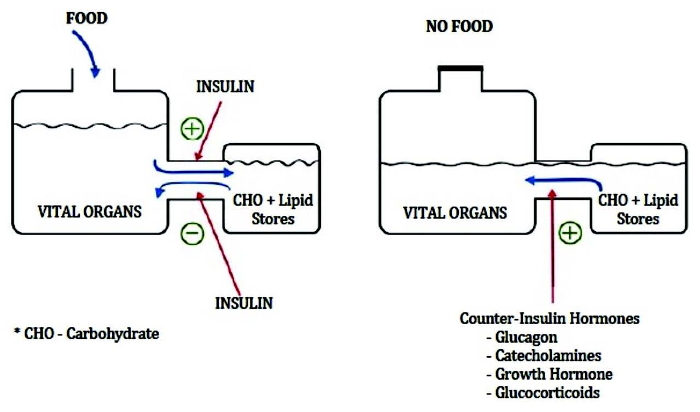
\includegraphics{images/017.jpg}
\end{figure}

ಹೀಗೆ ದೈಹಿಕ, ಮಾನಸಿಕ, \enginline{Neurophysiological, Endocrine and Metabolic} ಬದಲಾವಣೆಗಳನ್ನು ಅಳೆದು ನೋಡಲಿರುವ ವೈಜ್ಞಾನಿಕ ಮಾಪಕಗಳನ್ನು ಬಳಸಿಕೊಂಡು ಯೋಗಾಭ್ಯಾಸದ ಅಧ್ಯಯನ ಗೈಯಲಾಗಿದೆ.

ಆಸನ, ಪ್ರಾಣಾಯಾಮ ಮತ್ತು ಶವಾಸನಗಳ ಸಂಯುಕ್ತಾಭ್ಯಾಸವನ್ನು ಮೂರು ತಿಂಗಳವರೆಗೆ ನಡೆಸಿಕೊಂಡುಬಂದ ಸ್ವಯಂಸೇವಕರಲ್ಲಿ, ದೈಹಿಕ ಮತ್ತು ಜೀವರಾಸಾಯನಿಕ ಸುಧಾರಣೆಗಳು ಈ ಕೆಳಗೆ ವಿವರಿಸಿದಂತೆ ಕಂಡುಬಂದುವು:

\begin{center}
\enginline{\textbf{Showing the Physiological and Biochemical changesfollowing the three months course of the combined practice of Asanas, Pranayamas and Shavasana.}}
\end{center}


\begin{figure}
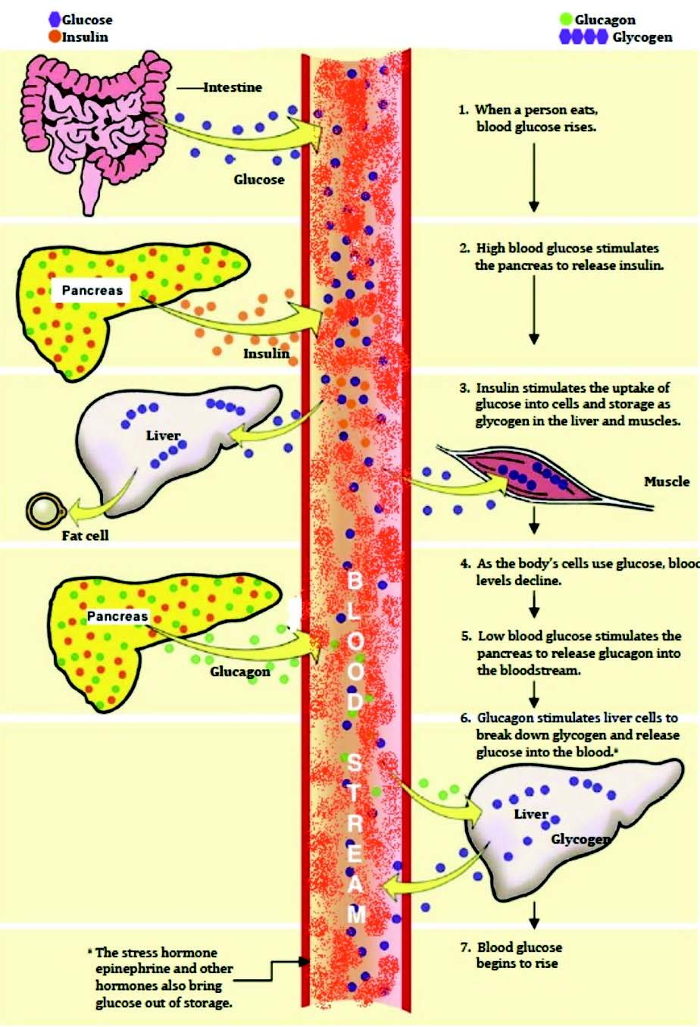
\includegraphics{images/018.jpg}
\end{figure}


\begin{figure}
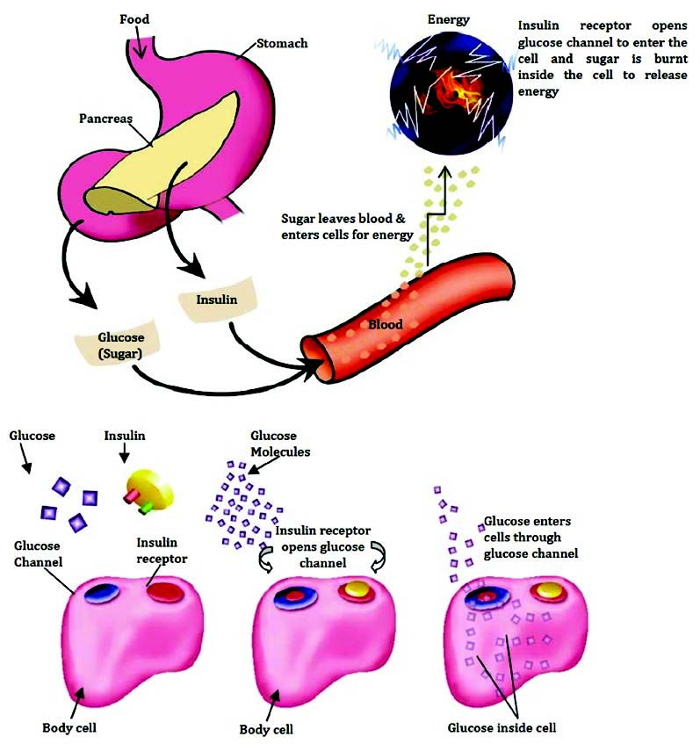
\includegraphics{images/019.jpg}
\caption{\textbf{ಚಿತ್ರ \general{\enginline{31:}} ಮೇಲೆ ಹೇಳಿದಂತೆ ಮೂರು ತರದ (ಆಸನ, ಪ್ರಾಣಾಯಾಮ, ಧ್ಯಾನ) ಯೋಗಾಭ್ಯಾಸದ ಫಲಿತಾಂಶಗಳ ಸಾರಾಂಶ.} }
\end{figure}

